% Options for packages loaded elsewhere
% Options for packages loaded elsewhere
\PassOptionsToPackage{unicode}{hyperref}
\PassOptionsToPackage{hyphens}{url}
\PassOptionsToPackage{dvipsnames,svgnames,x11names}{xcolor}
%
\documentclass[
  french,
  letterpaper,
  DIV=11,
  numbers=noendperiod]{scrreprt}
\usepackage{xcolor}
\usepackage{amsmath,amssymb}
\setcounter{secnumdepth}{5}
\usepackage{iftex}
\ifPDFTeX
  \usepackage[T1]{fontenc}
  \usepackage[utf8]{inputenc}
  \usepackage{textcomp} % provide euro and other symbols
\else % if luatex or xetex
  \usepackage{unicode-math} % this also loads fontspec
  \defaultfontfeatures{Scale=MatchLowercase}
  \defaultfontfeatures[\rmfamily]{Ligatures=TeX,Scale=1}
\fi
\usepackage{lmodern}
\ifPDFTeX\else
  % xetex/luatex font selection
\fi
% Use upquote if available, for straight quotes in verbatim environments
\IfFileExists{upquote.sty}{\usepackage{upquote}}{}
\IfFileExists{microtype.sty}{% use microtype if available
  \usepackage[]{microtype}
  \UseMicrotypeSet[protrusion]{basicmath} % disable protrusion for tt fonts
}{}
\makeatletter
\@ifundefined{KOMAClassName}{% if non-KOMA class
  \IfFileExists{parskip.sty}{%
    \usepackage{parskip}
  }{% else
    \setlength{\parindent}{0pt}
    \setlength{\parskip}{6pt plus 2pt minus 1pt}}
}{% if KOMA class
  \KOMAoptions{parskip=half}}
\makeatother
% Make \paragraph and \subparagraph free-standing
\makeatletter
\ifx\paragraph\undefined\else
  \let\oldparagraph\paragraph
  \renewcommand{\paragraph}{
    \@ifstar
      \xxxParagraphStar
      \xxxParagraphNoStar
  }
  \newcommand{\xxxParagraphStar}[1]{\oldparagraph*{#1}\mbox{}}
  \newcommand{\xxxParagraphNoStar}[1]{\oldparagraph{#1}\mbox{}}
\fi
\ifx\subparagraph\undefined\else
  \let\oldsubparagraph\subparagraph
  \renewcommand{\subparagraph}{
    \@ifstar
      \xxxSubParagraphStar
      \xxxSubParagraphNoStar
  }
  \newcommand{\xxxSubParagraphStar}[1]{\oldsubparagraph*{#1}\mbox{}}
  \newcommand{\xxxSubParagraphNoStar}[1]{\oldsubparagraph{#1}\mbox{}}
\fi
\makeatother


\usepackage{longtable,booktabs,array}
\newcounter{none} % for unnumbered tables
\usepackage{calc} % for calculating minipage widths
% Correct order of tables after \paragraph or \subparagraph
\usepackage{etoolbox}
\makeatletter
\patchcmd\longtable{\par}{\if@noskipsec\mbox{}\fi\par}{}{}
\makeatother
% Allow footnotes in longtable head/foot
\IfFileExists{footnotehyper.sty}{\usepackage{footnotehyper}}{\usepackage{footnote}}
\makesavenoteenv{longtable}
\usepackage{graphicx}
\makeatletter
\newsavebox\pandoc@box
\newcommand*\pandocbounded[1]{% scales image to fit in text height/width
  \sbox\pandoc@box{#1}%
  \Gscale@div\@tempa{\textheight}{\dimexpr\ht\pandoc@box+\dp\pandoc@box\relax}%
  \Gscale@div\@tempb{\linewidth}{\wd\pandoc@box}%
  \ifdim\@tempb\p@<\@tempa\p@\let\@tempa\@tempb\fi% select the smaller of both
  \ifdim\@tempa\p@<\p@\scalebox{\@tempa}{\usebox\pandoc@box}%
  \else\usebox{\pandoc@box}%
  \fi%
}
% Set default figure placement to htbp
\def\fps@figure{htbp}
\makeatother



\ifLuaTeX
\usepackage[bidi=basic,shorthands=off]{babel}
\else
\usepackage[bidi=default,shorthands=off]{babel}
\fi
\ifLuaTeX
  \usepackage{selnolig} % disable illegal ligatures
\fi


\setlength{\emergencystretch}{3em} % prevent overfull lines

\providecommand{\tightlist}{%
  \setlength{\itemsep}{0pt}\setlength{\parskip}{0pt}}



 


\KOMAoption{captions}{tableheading}
\makeatletter
\@ifpackageloaded{tcolorbox}{}{\usepackage[skins,breakable]{tcolorbox}}
\@ifpackageloaded{fontawesome5}{}{\usepackage{fontawesome5}}
\definecolor{quarto-callout-color}{HTML}{909090}
\definecolor{quarto-callout-note-color}{HTML}{0758E5}
\definecolor{quarto-callout-important-color}{HTML}{CC1914}
\definecolor{quarto-callout-warning-color}{HTML}{EB9113}
\definecolor{quarto-callout-tip-color}{HTML}{00A047}
\definecolor{quarto-callout-caution-color}{HTML}{FC5300}
\definecolor{quarto-callout-color-frame}{HTML}{acacac}
\definecolor{quarto-callout-note-color-frame}{HTML}{4582ec}
\definecolor{quarto-callout-important-color-frame}{HTML}{d9534f}
\definecolor{quarto-callout-warning-color-frame}{HTML}{f0ad4e}
\definecolor{quarto-callout-tip-color-frame}{HTML}{02b875}
\definecolor{quarto-callout-caution-color-frame}{HTML}{fd7e14}
\makeatother
\makeatletter
\@ifpackageloaded{bookmark}{}{\usepackage{bookmark}}
\makeatother
\makeatletter
\@ifpackageloaded{caption}{}{\usepackage{caption}}
\AtBeginDocument{%
\ifdefined\contentsname
  \renewcommand*\contentsname{Table des matières}
\else
  \newcommand\contentsname{Table des matières}
\fi
\ifdefined\listfigurename
  \renewcommand*\listfigurename{Liste des Figures}
\else
  \newcommand\listfigurename{Liste des Figures}
\fi
\ifdefined\listtablename
  \renewcommand*\listtablename{Liste des Tables}
\else
  \newcommand\listtablename{Liste des Tables}
\fi
\ifdefined\figurename
  \renewcommand*\figurename{Figure}
\else
  \newcommand\figurename{Figure}
\fi
\ifdefined\tablename
  \renewcommand*\tablename{Table}
\else
  \newcommand\tablename{Table}
\fi
}
\@ifpackageloaded{float}{}{\usepackage{float}}
\floatstyle{ruled}
\@ifundefined{c@chapter}{\newfloat{codelisting}{h}{lop}}{\newfloat{codelisting}{h}{lop}[chapter]}
\floatname{codelisting}{Listing}
\newcommand*\listoflistings{\listof{codelisting}{Liste des Listings}}
\usepackage{amsthm}
\theoremstyle{plain}
\newtheorem{theorem}{Théorème}[chapter]
\theoremstyle{definition}
\newtheorem{definition}{Définition}[chapter]
\theoremstyle{plain}
\newtheorem{lemma}{Lemme}[chapter]
\theoremstyle{plain}
\newtheorem{proposition}{Proposition}[chapter]
\theoremstyle{definition}
\newtheorem{exercise}{Exercice}[chapter]
\theoremstyle{definition}
\newtheorem{example}{Exemple}[chapter]
\theoremstyle{remark}
\AtBeginDocument{\renewcommand*{\proofname}{Preuve}}
\newtheorem*{remark}{Remarque}
\newtheorem*{solution}{Solution}
\newtheorem{refremark}{Remarque}[chapter]
\newtheorem{refsolution}{Solution}[chapter]
\makeatother
\makeatletter
\makeatother
\makeatletter
\@ifpackageloaded{caption}{}{\usepackage{caption}}
\@ifpackageloaded{subcaption}{}{\usepackage{subcaption}}
\makeatother
\newcounter{quartocalloutnteno}
\newcommand{\quartocalloutnte}[1]{\refstepcounter{quartocalloutnteno}\label{#1}}
\newcounter{quartocalloutwrnno}
\newcommand{\quartocalloutwrn}[1]{\refstepcounter{quartocalloutwrnno}\label{#1}}
\newcounter{quartocallouttipno}
\newcommand{\quartocallouttip}[1]{\refstepcounter{quartocallouttipno}\label{#1}}
\usepackage{bookmark}
\IfFileExists{xurl.sty}{\usepackage{xurl}}{} % add URL line breaks if available
\urlstyle{same}
\hypersetup{
  pdftitle={Mathématiques en TSI2},
  pdfauthor={Pierre Pageault},
  pdflang={fr},
  colorlinks=true,
  linkcolor={blue},
  filecolor={Maroon},
  citecolor={Blue},
  urlcolor={Blue},
  pdfcreator={LaTeX via pandoc}}


\title{Mathématiques en TSI2}
\author{Pierre Pageault}
\date{2026-09-10}
\begin{document}
\maketitle

\renewcommand*\contentsname{Table des matières}
{
\setcounter{tocdepth}{2}
\tableofcontents
}

\bookmarksetup{startatroot}

\chapter*{Preface}\label{preface}
\addcontentsline{toc}{chapter}{Preface}

\markboth{Preface}{Preface}

Ce document contient les documents pédagogiques relatifs au cours de
mathématiques de deuxième année dispensé en TSI2 au lycée Etienne Mimard
de Saint Etienne.

\bookmarksetup{startatroot}

\chapter{Intégrales
généralisées}\label{intuxe9grales-guxe9nuxe9ralisuxe9es}

\section*{Introduction}\label{introduction}
\addcontentsline{toc}{section}{Introduction}

\markright{Introduction}

Le but de ce chapitre est de généralisée la théorie de l'intégration vue
en première année -- qui se limite à des segments -- à des intervalles
\emph{quelconques} . On donnera par exemple un sens à des intégrales
comme \(\displaystyle\int_{1}^{\infty}\frac{dx}{x^{2}}\) ou
\(\displaystyle\int_{0}^{1}\ln(x)dx\).

La théorie de l'intégration vue en première année est héritée de
Riemann\footnote{Georg Friedrich Bernhard Riemann, mathématicien
  Allemand né le 17 septembre 1826 à Breselenz, et mort le 20 juillet
  1866 à Selasca, en Italie.} qui l'introduit dans son article fondateur
« Über die Darstellbarkeit einer Function durch eine trigonometrische
Reihe » (Sur la représentabilité d'une fonction par une série
trigonométrique) en 1854.

L'intégrale y est définie via des \emph{sommes}, qui portent aujourd'hui
le nom de \emph{sommes de Riemann}.

\begin{figure}

\centering{

\pandocbounded{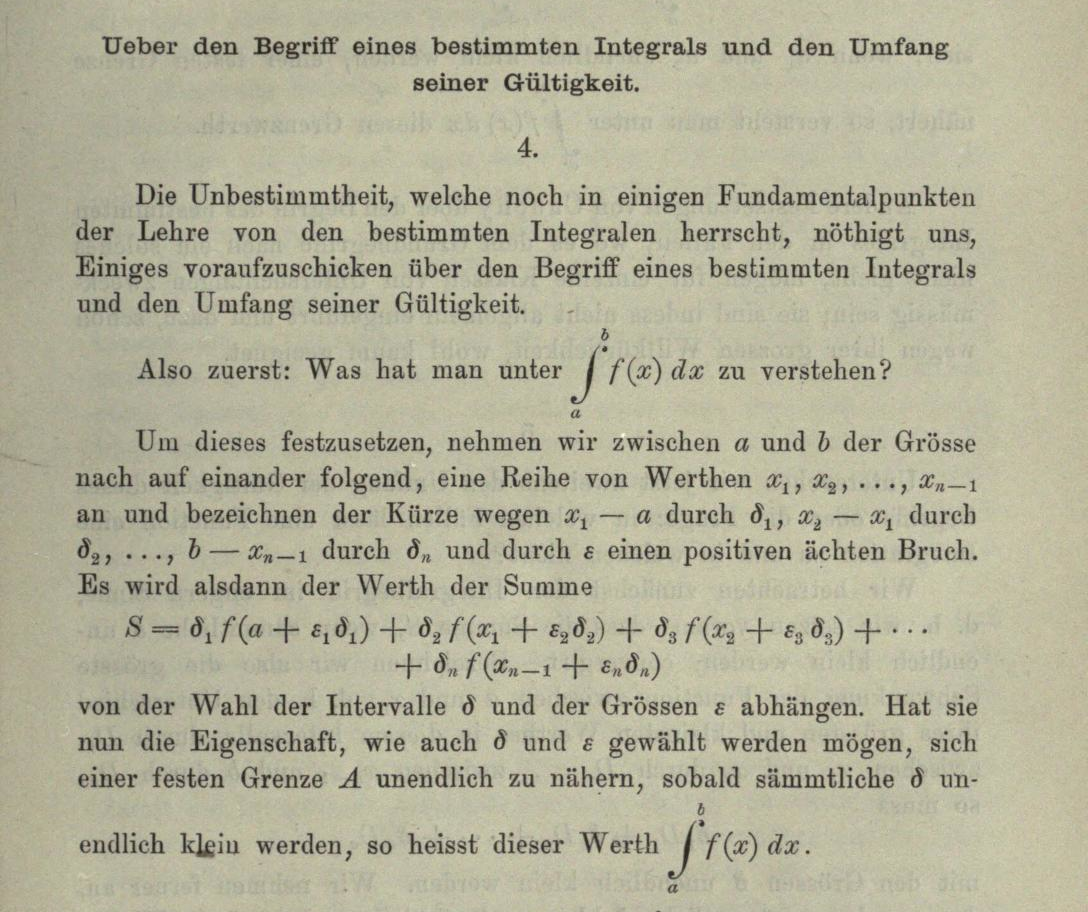
\includegraphics[keepaspectratio]{./png/somme-riemann.png}}

}

\caption{\label{fig-somme-riemann}La définition initiale de Riemann de
l'intégrale à l'aide de sommes.}

\end{figure}%

L'énoncé moderne correspondant est le suivant:

\begin{definition}[Sommes de
Riemann]\protect\hypertarget{def-somme-riemann}{}\label{def-somme-riemann}

Soit \(f:[a,b] \to \mathbb{R}\) une fonction continue sur \([a,b]\),
avec \(a,b \in
\mathbb{R}\), \(a \leqslant b\). Pour tout \(n \geqslant 1\), on définit

\[
    U_{n} = \frac{b-a}{n}\sum_{k=0}^{n-1}f \left(a + k \frac{b-a}{n}\right)
\]

et

\[
   V_{n} = \frac{b-a}{n} \sum_{k=1}^{n} f \left(a+ k \frac{b-a}{n}\right). 
\]

Alors les suites \((U_{n})\) et \((V_{n})\) convergent vers une limite
commune appelée intégrale de \(f\) sur \([a,b]\) et notée
\(\int_a^b f(t)dt\).

\end{definition}

On peut montrer alors que la fonction \(x \mapsto \int_a^x f(t)dt\) est
une \emph{primitive} de \(f\) sur \([a,b]\) et on aboutit à la
définition usuelle de l'intégrale donnée en première année : pour toute
primitive \(F\) de \(f\) sur \([a,b]\),

\[
    \int_{a}^{b}f(t)dt = F(b)-F(a).
\]

Puisque qu'une telle primitive \(F\) est nécessairement continue sur
\([a,b]\) (elle y est de classe \(C^{1}\)), on a en particulier

\[
    \int_{a}^{b}f(t)dt = \lim_{x \to b^-} \int_{a}^{x}f(t)dt.
\]

Cette relation présente l'avantage de garder éventuellement un sens
lorsque \(f\) n'est pas définie en \(b\), par exemple lorque
\(b=+\infty\) ; on parlera alors d'intégrale \emph{généralisée} de \(f\)
sur \([a,b[\).

Les intégrales généralisées seront donc définies comme des
\emph{limites} d'intégrales usuelles -- à condition que ces limites
existent ! Contrairement aux intégrales usuelles, les intégrales
généralisées ne seront donc pas toujours bien définies, et il faudra
prendre plus de précaution lors de leurs manipulations.

Ces précautions étant prises, les intégrales généralisées se
comporteront essentiellement de la même manière que les intégrales
usuelles.

Les intégrales généralisées sont d'un usuage constant en mathématiques
et en physique (transformée de Laplace, de Fourier, fonction \(\Gamma\)
d'Euler, intégrale de Gauss,\ldots)

\section{Convergence d'un intégrale généralisée}\label{sec-convergence}

Dans tout ce chapitre, \(I\) désigne un intervalle non vide de
\(\mathbb{R}\), d'extrémités
\(a,b \in \mathbb{R}\cup \left\{ \pm \infty\right\}\), avec \(a
\leqslant b\), et \(\mathbb{K}\) désigne \(\mathbb{R}\) ou
\(\mathbb{C}\).

\subsection{Intégrales
généralisées}\label{intuxe9grales-guxe9nuxe9ralisuxe9es-1}

\begin{definition}[]\protect\hypertarget{def-integrale-generalisee}{}\label{def-integrale-generalisee}

Soit \(f:I \to \mathbb{K}\) une fonction \emph{continue} sur \(I\) et
\(\alpha\) une extrémité de \(I\). On dit que l'intégrale de \(f\) sur
\(I\) est \textbf{généralisée en \(\boldsymbol{\alpha}\)} si \(I\) est
\emph{ouvert} en \(\alpha\). On dit que l'intérgrale de \(f\) sur \(I\)
est \textbf{généralisée} si elle est généralisée en au moins une des
extrémités de \(I\).

\end{definition}

\begin{tcolorbox}[enhanced jigsaw, arc=.35mm, bottomrule=.15mm, bottomtitle=1mm, breakable, colback=white, colbacktitle=quarto-callout-note-color!10!white, colframe=quarto-callout-note-color-frame, coltitle=black, left=2mm, leftrule=.75mm, opacityback=0, opacitybacktitle=0.6, rightrule=.15mm, title=\textcolor{quarto-callout-note-color}{\faInfo}\hspace{0.5em}{Note \ref*{nte-ambiguite}}, titlerule=0mm, toprule=.15mm, toptitle=1mm]

\quartocalloutnte{nte-ambiguite} 

La phrase ``l'intégrale de \(f\) sur \(I\)'' s'abrège usuellement
\(\int_{I}f\), \(\int_{I}f(t)dt\) ou \(\int_{a}^{b}f(t)dt\). Il faut
noter l'\emph{ambiguité} de cette dernière notation (qui est pourtant la
plus utilisée) car elle ne précise pas si les bornes \(a\) et \(b\) sont
inclues ou exclues. C'est justement à vous que revient de lever cette
ambiguité pour étudier l'aspect généralisé ou non de l'intégrale.

\end{tcolorbox}

\begin{example}[]\protect\hypertarget{exm-simplement-generalisee-1}{}\label{exm-simplement-generalisee-1}

L'intégrale \(\int_{1}^{+\infty}\frac{dx}{x^2}\) est généralisée en
\(+\infty\) uniquement car la fonction \(x \mapsto \frac{1}{x^{2}}\) est
continue sur \([1,+\infty[\).

\end{example}

\begin{example}[]\protect\hypertarget{exm-simplement-generalisee-3}{}\label{exm-simplement-generalisee-3}

L'intégrale \(\int_{0}^{1}\frac{\ln(t)}{1-t}dt\) est généralisée en
\(0\) et en \(1\) car la fonction \(t \mapsto \frac{\ln(t)}{1-t}\) est
continue sur \(]0,1[\). On dit qu'elle est \emph{doublement}
généralisée.

\end{example}

\begin{tcolorbox}[enhanced jigsaw, arc=.35mm, bottomrule=.15mm, bottomtitle=1mm, breakable, colback=white, colbacktitle=quarto-callout-tip-color!10!white, colframe=quarto-callout-tip-color-frame, coltitle=black, left=2mm, leftrule=.75mm, opacityback=0, opacitybacktitle=0.6, rightrule=.15mm, title=\textcolor{quarto-callout-tip-color}{\faLightbulb}\hspace{0.5em}{Astuce}, titlerule=0mm, toprule=.15mm, toptitle=1mm]

L'aspect généralisée d'une intégrale se lit sur le \emph{domaine} de la
fonction intégrée.

\end{tcolorbox}

Que dire maintenant de l'intégrale de la fonction \(x \mapsto x^{2}\)
sur l'intervalle \(]0,1]\) ? Certe l'extrémité gauche est ouverte mais
la fonction \(x
\mapsto x^{2}\) est continue sur \([0,1]\)\ldots{} On peut de même se
poser la question de l'intégrale de la fonction \(x \mapsto x\ln(x)\)
sur l'intervalle \(]0,1]\) qui se \emph{prolonge par continuité} en
\(0\). Ces situations correspondent au cas des intégrales
\emph{faussement généralisées}, étudiées plus en détail dans la
Section~\ref{sec-integrale-faussement-generalisee}.

\subsection{Convergence d'une intégrale
généralisée}\label{convergence-dune-intuxe9grale-guxe9nuxe9ralisuxe9e}

Jusqu'à présent, on s'est seulement entendu sur le sens de la phrase
``l'intégrale de \(f\) sur \(I\) est généralisée''. Nous pas attribué de
\emph{valeur numérique} à cette ``intégrale''. C'est le rôle de la
notion de \emph{convergence}.

\begin{definition}[Cas d'un intervalle semi ouvert à
droite]\protect\hypertarget{def-cv-integrale-intervalle-semi-ouvert}{}\label{def-cv-integrale-intervalle-semi-ouvert}

Soit \(f:[a,b[ \to \mathbb{K}\) une fonction continue. On dit que
l'intégrale de \(f\) sur \([a,b[\) \textbf{converge} si l'intégrale
partielle \(\int_{a}^{x}f(t)dt\) admet une limite \emph{finie} quand
\(x \to b^-\). On pose alors \[
\boxed{
    \int_{a}^{b}f(t)dt \underset{\small \mathrm{def}}{=}\lim_{x \to b^-}
\int_{a}^{x}f(t)dt}
\] Dans le cas contraire, on dit que l'intégrale de \(f\) sur \(I\)
\textbf{diverge}. La convergence ou la divergence d'une intégrale
s'appelle sa \textbf{nature}.

\end{definition}

\begin{figure}

\centering{

\pandocbounded{
\includegraphics[keepaspectratio]{index_files/mediabag/tikz/svg/01-1a.pdf}}

}

\caption{\label{fig-integrale-partielle-droite}Intégrale partielle et
généralisée dans le cas \(b=+\infty\).}

\end{figure}%

\begin{tcolorbox}[enhanced jigsaw, arc=.35mm, bottomrule=.15mm, bottomtitle=1mm, breakable, colback=white, colbacktitle=quarto-callout-note-color!10!white, colframe=quarto-callout-note-color-frame, coltitle=black, left=2mm, leftrule=.75mm, opacityback=0, opacitybacktitle=0.6, rightrule=.15mm, title=\textcolor{quarto-callout-note-color}{\faInfo}\hspace{0.5em}{Note \ref*{nte-existe}}, titlerule=0mm, toprule=.15mm, toptitle=1mm]

\quartocalloutnte{nte-existe} 

On dit aussi qu'une intégrale généralisée \textbf{bien définie} ou
\textbf{existe} (en référence à la limite qui la définie) pour signifier
qu'elle \emph{converge} ; ce sont des synonymes.

\end{tcolorbox}

\begin{example}[]\protect\hypertarget{exm-riemann-1}{}\label{exm-riemann-1}

L'intégrale \(\int_{1}^{+\infty}\frac{dx}{x^{2}}\) converge et vaut
\(1\).

Pour tout \(x \geqslant 1\), on a

\[
    \int_{1}^{x}\frac{dt}{t^{2}} = 1- \frac{1}{x} \underset{x \to +\infty}{\longrightarrow} 1.
\]

Donc l'intégrale \(\int_{1}^{+\infty}\frac{dx}{x^{2}}\) converge et vaut
\(1\).

\end{example}

\begin{example}[]\protect\hypertarget{exm-riemann-3}{}\label{exm-riemann-3}

L'intégrale \(\int_{1}^{+\infty}\frac{dx}{x}\) diverge.

Pour tout \(x \geqslant 1\), on a

\[
    \int_{1}^{x}\frac{dt}{t} = \ln(x) \underset{x \to +\infty}{\longrightarrow} +\infty,
\]

donc l'intégrale \(\int_{1}^{+\infty}\frac{dx}{x}\) diverge.

\end{example}

\begin{refremark}
Les exemples précédents montrent qu'il ne faut pas confondre la
convergence en \(+\infty\) de l'\emph{intégrale} et de la \emph{fonction
intégrée} (l'intégrande). Par exemple, la fonction \(x \mapsto 1/x\)
admet une limite en \(+\infty\), mais l'intégrale
\(\int_{1}^{+\infty}\frac{dx}{x}\) diverge.

\label{rem-convergence-integrande}

\end{refremark}

\begin{figure}

\begin{minipage}[t]{0.50\linewidth}

\raisebox{-\height}{

\pandocbounded{
\includegraphics[keepaspectratio]{index_files/mediabag/tikz/svg/01-5a.pdf}}

}

\end{minipage}%
%
\begin{minipage}[t]{0.50\linewidth}

\raisebox{-\height}{

\pandocbounded{
\includegraphics[keepaspectratio]{index_files/mediabag/tikz/svg/01-5b.pdf}}

}

\end{minipage}%

\caption{\label{fig-riemann-2}Des fonctions peuvent avoir des graphes
similaires mais des intégrales de nature tout à fait différente.}

\end{figure}%

\begin{tcolorbox}[enhanced jigsaw, arc=.35mm, bottomrule=.15mm, bottomtitle=1mm, breakable, colback=white, colbacktitle=quarto-callout-warning-color!10!white, colframe=quarto-callout-warning-color-frame, coltitle=black, left=2mm, leftrule=.75mm, opacityback=0, opacitybacktitle=0.6, rightrule=.15mm, title=\textcolor{quarto-callout-warning-color}{\faExclamationTriangle}\hspace{0.5em}{Avertissement \ref*{wrn-convergence-integrande}}, titlerule=0mm, toprule=.15mm, toptitle=1mm]

\quartocalloutwrn{wrn-convergence-integrande} 

Il ne pas confondre la convergence de l'\emph{intégrale} en
\(\pm \infty\) et la convergence de la fonction intégrée
(l'\emph{intégrande}).

\end{tcolorbox}

Voici un autre exemple classique d'intégrale convergente.

\begin{example}[]\protect\hypertarget{exm-exponentielle}{}\label{exm-exponentielle}

L'intégrale \(\int_{0}^{+\infty}e^{-t}dt\) converge et vaut \(1\).

Pour tout \(x \geqslant 0\), on

\[
    \int_{0}^{x}e^{-t}dt = 1-e^{-x} \underset{x \to +\infty}{\longrightarrow} 1.
\]

Donc l'intégrale \(\int_{0}^{+\infty}e^{-t}dt\) converge et vaut \(1\).

\end{example}

\begin{refremark}
On définit de même la convergence d'une intégrale sur un intervalle semi
ouvert à gauche \(]a,b]\) en considérant les intégrales partielles
\(\int_{x}^{b}f(t)dt\) quand \(x \to a^{+}\) et en posant, en cas de
convergence

\[
\boxed{
    \int_{a}^{b}f(t)dt \underset{\small \mathrm{def}}{=}\lim_{x \to a^+}
\int_{x}^{b}f(t)dt}
\]

\label{rem-semi-ouvert-a-gauche}

\end{refremark}

\begin{figure}

\centering{

\pandocbounded{
\includegraphics[keepaspectratio]{index_files/mediabag/tikz/svg/01-1b.pdf}}

}

\caption{\label{fig-convergence-ouvert-gauche}Intégrale partielle et
intégrable généralisée dans le cas \(a=0\).}

\end{figure}%

\begin{example}[]\protect\hypertarget{exm-riemann-2}{}\label{exm-riemann-2}

L'intégrale \(\int_{0}^{1}\frac{dx}{x^{2}}\) diverge.

Pour tout \(\varepsilon>0\), on a

\[
    \int_{\varepsilon}^{1}\frac{dx}{x^{2}} = \frac{1}{\varepsilon}-1 \underset{\varepsilon \to 0^{+}}{\longrightarrow} +\infty.
\]

Donc l'intégrale \(\int_{0}^{1}\frac{dx}{x^{2}}\) diverge.

\end{example}

On vient d'associer à certaine intégrales une valeur numérique. On va
donc pouvoir commencer à \emph{calculer} avec des intégrales
généralisées. Ce point sera abordé plus en détail dans la
Section~\ref{sec-calculer} mais nous énonçons dès maintenant la
\emph{relation de Chasles}, attendue de toute théorie satisfaisante de
l'intégration.

\begin{proposition}[Relation de Chasles sur un intervalle semi
ouvert]\protect\hypertarget{prp-Chasles-semi-ouvert-droite}{}\label{prp-Chasles-semi-ouvert-droite}

Soit \(f:[a,b[ \to \mathbb{K}\) une fonction continue. Alors pour tout
point \(c \in [a,b[\), les intégrales \(\int_{a}^{b}f(t)dt\) et
\(\int_{c}^{b}f(t)dt\) ont \emph{même nature} et, \emph{en cas de
convergence}, on a \[
\int_{a}^{b}f(t)dt = \int_{a}^{c}f(t)dt + \int_{c}^{b}f(t)dt.
\]

\end{proposition}

\begin{tcolorbox}[enhanced jigsaw, arc=.35mm, bottomrule=.15mm, bottomtitle=1mm, breakable, colback=white, colbacktitle=quarto-callout-tip-color!10!white, colframe=quarto-callout-tip-color-frame, coltitle=black, left=2mm, leftrule=.75mm, opacityback=0, opacitybacktitle=0.6, rightrule=.15mm, title=\textcolor{quarto-callout-tip-color}{\faLightbulb}\hspace{0.5em}{Astuce \ref*{tip-chasles}}, titlerule=0mm, toprule=.15mm, toptitle=1mm]

\quartocallouttip{tip-chasles} 

Si elles sont généralisées uniquement en \(b\), les intégrales
\(\int_{a}^{b}f(t)dt\) et \(\int_{c}^{b}f(t)dt\) ont \emph{même nature}.

\end{tcolorbox}

\begin{refremark}
La Proposition~\ref{prp-Chasles-semi-ouvert-droite} et le
Tip~\ref{tip-chasles} se généralisent naturellement au cas d'un
intervalle semi ouvert à gauche \(]a,b]\).

\label{rem-version-semi-ouvert-gauche}

\end{refremark}

Une fois la convergence définie dans le cas d'intervalles semi ouverts,
la relation de Chasles -- que l'on veut valide pour les intégrales
généralisées -- suggère la définition suivante dans le cas d'un
intervalle ouvert.

\begin{definition}[Cas d'un intervalle
ouvert]\protect\hypertarget{def-cv-intervalle-ouvert}{}\label{def-cv-intervalle-ouvert}

Soit \(f:]a,b[ \to \mathbb{K}\) une fonction continue. On dit que
l'intégrale de \(f\) sur \(]a,b[\) \textbf{converge} si elle converge
\textbf{en \(\boldsymbol{a}\)} \emph{et} en \textbf{en
\(\boldsymbol{b}\)}, c.à.d s'il existe un réel \(c \in ]a,b[\), tel que
les \emph{deux} intégrales \(\int_{a}^{c}f(t)dt\) et
\(\int_{c}^{b}f(t)dt\) convergent. On pose alors

\[
\int_{a}^{b}f(t)dt \underset{\mathrm{def}}{=}
\int_{a}^{c}f(t)dt + \int_{c}^{b}f(t)dt. 
\]

Dans le cas contraire, on dit que l'intégrale de \(f\) sur \(]a,b[\)
\textbf{diverge}. La convergence ou la divergence d'une intégrale
s'appelle sa \textbf{nature}.

\end{definition}

\begin{refremark}
Cette définition et la valeur de l'intégrale ne dépendent pas du point
\(c\) utilisé par la relation de Chasles satisfaite par les intégrales
généralisées sur un intervalle semi ouvert
(Proposition~\ref{prp-Chasles-semi-ouvert-droite}).

\label{rem-chasles}

\end{refremark}

\begin{example}[]\protect\hypertarget{exm-ouvert-convergente}{}\label{exm-ouvert-convergente}

L'intégrale \(\int_{-\infty}^{+\infty}\frac{dx}{1+x^{2}}\) converge et
vaut \(\pi\).

Pour tout \(w \geqslant 0\), on a

\[
    \int_{0}^{x}\frac{dt}{1+t^{2}}= \arctan(x) \underset{x \to+\infty}{\longrightarrow} \frac{\pi}{2}.
\]

Donc l'intégrale \(\int_{0}^{+\infty}\frac{dx}{1+x^{2}}\) converge et
vaut \(\pi/2\).

De même, pour tout \(x \leqslant 0\), on a

\[
    \int_{x}^{0}\frac{dt}{1+t^{2}} = - \arctan(x) \underset{x \to -\infty}{\longrightarrow} \frac{\pi}{2}.
\]

Donc par \emph{définition} l'intégrale
\(\int_{-\infty}^{+\infty}\frac{dx}{1+x^{2}}\) converge et vaut \(\pi\).

\end{example}

\begin{example}[]\protect\hypertarget{exm-ouvert-divergente}{}\label{exm-ouvert-divergente}

L'intégrale \(\int_{0}^{+\infty}\frac{dx}{x^{2}}\) diverge car elle
diverge en \(0\).

\end{example}

\begin{tcolorbox}[enhanced jigsaw, arc=.35mm, bottomrule=.15mm, bottomtitle=1mm, breakable, colback=white, colbacktitle=quarto-callout-tip-color!10!white, colframe=quarto-callout-tip-color-frame, coltitle=black, left=2mm, leftrule=.75mm, opacityback=0, opacitybacktitle=0.6, rightrule=.15mm, title=\textcolor{quarto-callout-tip-color}{\faLightbulb}\hspace{0.5em}{Astuce \ref*{tip-ouvert}}, titlerule=0mm, toprule=.15mm, toptitle=1mm]

\quartocallouttip{tip-ouvert} 

Montrer la convergence d'une intégrale sur un espace \emph{ouvert},
c'est montrer la convergence de \emph{deux} intégrales ``simplement''
généralisées.

\end{tcolorbox}

\subsection{Intégrales faussement
généralisées}\label{sec-integrale-faussement-generalisee}

Nous traitons ici le cas des intégrales dites \emph{faussement
généralisées}, comme \(\int_{]0,1]}x^{2}dx\) ou
\(\int_{]0,1]}x\ln(x)dx\), très fréquentes en pratique.

L'intuition voudrait que ces intégrales soient convergentes, et que la
valeur de l'intégrale ne dépende pas de l'inclusion ou de l'exclusion
des bornes de l'intégrale car ``il n'y a pas d'aire sous un point''. La
Proposition~\ref{prp-integrale-faussement-generalisee} montre que c'est
effectivement le cas.

\begin{definition}[]\protect\hypertarget{def-faussement-generalisee}{}\label{def-faussement-generalisee}

Soit \(f:I \to \mathbb{K}\) une fonction continue et \(\alpha\) une
extrémité ouverte de \(I\). On dit que l'intégrale de \(f\) sur \(I\)
est \textbf{faussement généralisée en \(\boldsymbol{\alpha}\)} si \(f\)
se prolonge par continuité en \(\alpha\). On dit que l'intégrale de
\(f\) sur \(I\) est \textbf{faussement généralisée} si \(f\) se prolonge
par continuité en chaque extrémité ouverte de \(I\).

\end{definition}

La note suivante est à comparer au
Warning~\ref{wrn-convergence-integrande}.

\begin{tcolorbox}[enhanced jigsaw, arc=.35mm, bottomrule=.15mm, bottomtitle=1mm, breakable, colback=white, colbacktitle=quarto-callout-note-color!10!white, colframe=quarto-callout-note-color-frame, coltitle=black, left=2mm, leftrule=.75mm, opacityback=0, opacitybacktitle=0.6, rightrule=.15mm, title=\textcolor{quarto-callout-note-color}{\faInfo}\hspace{0.5em}{Note \ref*{nte-borne-finie}}, titlerule=0mm, toprule=.15mm, toptitle=1mm]

\quartocalloutnte{nte-borne-finie} 

Le prolongement par continuité est réservé aux extrémités \emph{finies}
de \(I\). On ne peut donc par parler d'intégrales ``faussement
généralisées en \(\pm\infty\)'' lorsque la fonction intégrée admet une
limite finie en \(\pm \infty\).

\end{tcolorbox}

\begin{example}[]\protect\hypertarget{exm-integrale-faussement-generalisee}{}\label{exm-integrale-faussement-generalisee}

Les intégrales \(\int_{]0,1]}x^{2}dx\) et \(\int_{]0,1]}x\ln(x)dx\) sont
toutes les deux faussement généralisées en \(0\) car \(x^{2} \to 0\)
quand \(x \to
0^{+}\) et \(x\ln(x) \to 0\) quand \(x \to 0^{+}\) par \emph{croissance
comparée}.

\end{example}

\begin{proposition}[Convergence des intégrales faussement
généralisées]\protect\hypertarget{prp-integrale-faussement-generalisee}{}\label{prp-integrale-faussement-generalisee}

Si l'intégrale de \(f\) sur \(I\) est faussement généralisée, elle est
convergente et

\[
\int_I f = \int_{\bar{I}} f.
\]

\end{proposition}

\begin{tcolorbox}[enhanced jigsaw, arc=.35mm, bottomrule=.15mm, bottomtitle=1mm, breakable, colback=white, colbacktitle=quarto-callout-note-color!10!white, colframe=quarto-callout-note-color-frame, coltitle=black, left=2mm, leftrule=.75mm, opacityback=0, opacitybacktitle=0.6, rightrule=.15mm, title=\textcolor{quarto-callout-note-color}{\faInfo}\hspace{0.5em}{Note \ref*{nte-adherence}}, titlerule=0mm, toprule=.15mm, toptitle=1mm]

\quartocalloutnte{nte-adherence} 

Ici, \(\bar{I}\) désigne l'\emph{adhérence} de l'intervalle \(I\) ; il
s'agit du même intervalle dans lequel on a refermé toutes les bornes
ouvertes différentes de \(\pm \infty\).

\end{tcolorbox}

\begin{tcolorbox}[enhanced jigsaw, arc=.35mm, bottomrule=.15mm, bottomtitle=1mm, breakable, colback=white, colbacktitle=quarto-callout-note-color!10!white, colframe=quarto-callout-note-color-frame, coltitle=black, left=2mm, leftrule=.75mm, opacityback=0, opacitybacktitle=0.6, rightrule=.15mm, title=\textcolor{quarto-callout-note-color}{\faInfo}\hspace{0.5em}{Note \ref*{nte-prolongement}}, titlerule=0mm, toprule=.15mm, toptitle=1mm]

\quartocalloutnte{nte-prolongement} 

Dans le théorème précédent, le prolongement par continuité de \(f\) à
\(\bar{I}\) est encore noté \(f\). La rigueur voudrait qu'on le note
d'une autre manière, mais l'usage prévaut.

C'est l'occasion de rappeler qu'en mathématiques, une fonction vient
toujours avec un espace de \emph{départ} et un espace d'\emph{arrivée},
dont dépendent ses propriétés (injectivité, surjectivité,
régularité,\ldots). Les changer, c'est changer de fonction.

Bien souvent, on ``oublie'' ces espaces pour ne préciser que
l'\emph{action} de \(f\) ; ils sont alors présents de manière
\emph{sous-jaccente}.

\end{tcolorbox}

\begin{example}[]\protect\hypertarget{exm-faussement-generalisee}{}\label{exm-faussement-generalisee}

Les intégrales \(\int_{]0,1]}x^{2}dx\) et \(\int_{]0,1]}x\ln(x)dx\) sont
toutes les deux convergentes et on peut noter sans ambiguité leur valeur
\(\int_{0}^{1}x^{2}dx\) et \(\int_{0}^{1}x\ln(x)dx\).

\end{example}

\section{Les théorèmes de comparaison}\label{sec-comparaison}

Les seules intégrales réellement intéressantes sont les intégrales
convergentes. Actuellement, nous disposons d'un seul outil pour montrer
la convergence d'une intégrale généralisée : revenir à une intégrale
partielle et espérer être capable de la calculer pour étudier sa limite.

Malheureusement, peu d'intégrales sont effectivement calculables car il
est difficile de calculer des primitives, voir impossible\footnote{Un
  théorème de Liouville affirme par exemple qu'il n'existe pas de
  primitive de la fonction \(t \mapsto
  e^{-t^{2}}\) exprimable à l'aide de fonctions usuelles (polynômes,
  exponentielles, logarithmes, trigonométriques).}.

Face à ce constat, il est nécessaire de développer des outils permettant
de montrer qu'une intégrale converge sans pour autant calculer
explicitement une primitive de la fonction intégrée ; c'est le rôle des
théorèmes de comparaison.

\subsection{Le théorème de comparaison pour les fonctions
positives}\label{le-thuxe9oruxe8me-de-comparaison-pour-les-fonctions-positives}

Tous les théorèmes de comparaison que nous allons démontrer sont basés
sur le théorème suivant, lui même conséquence du théorème de la limite
monotone, qui est un théorème abstrait d'existence de \emph{limites}.

\begin{theorem}[Comparaison à l'aide de la relation \(\leqslant\) pour
les fonctions
positives]\protect\hypertarget{thm-comparaison-relation-leqslant}{}\label{thm-comparaison-relation-leqslant}

Soient \(f,g:I\to \mathbb{R}\) des fonctions continues sur \(I\). On
suppose que

\begin{enumerate}
\def\labelenumi{\arabic{enumi}.}
\tightlist
\item
  \(\forall t \in I,\ 0 \leqslant f(t) \leqslant g(t),\)
\item
  l'intégrale de \(g\) sur \(I\) converge.
\end{enumerate}

Alors l'intégrale de \(f\) sur \(I\) converge.

\end{theorem}

\begin{refremark}
Le théorème de comparaison permet donc un \emph{transfert de
technicité}; on passe d'un calcul de \emph{primitive} à une
\emph{majoration}.

\label{rem-transfert-technique}

\end{refremark}

\begin{example}[]\protect\hypertarget{exm-comparaison-fonction-positive}{}\label{exm-comparaison-fonction-positive}

Nature de l'intégrale \(\int_{0}^{+\infty}\frac{1- \cos(t)}{t^{2}}dt\).

L'intégrale proposée est généralisée en \(0\) et en \(+\infty\) car la
fonction \(t
\mapsto \frac{1- \cos(t)}{t^{2}}\) est continue sur \(]0,+\infty[\). Un
développement limité montre que cette intégrale est faussement
généralisée en \(0\) car

\[
    \frac{1- \cos(t)}{t^{2}} = \frac{t^{2}/2 + o(t^{2)}}{t^{2}} \sim \frac{1}{2}
\underset{t \to 0^{+}}{\longrightarrow} \frac{1}{2}.
\]

De plus, on a

\[
    \forall t \geqslant 1,\ 0 \leqslant \frac{1- \cos(t)}{t^{2}} \leqslant
\frac{2}{t^{2}}\tag{1},
\]

et l'intégrale \(\int_{1}^{+\infty}\frac{dt}{t^{2}}\) converge. Donc par
compraison de fonctions \emph{positives}, l'intégrale
\(\int_{0}^{+\infty}\frac{1 - \cos(t)}{t^{2}}dt\) converge en
\(+\infty\)\footnote{On utilise ici implicitement la linéarité de
  l'intégrale convergente : si l'intégrale de \(f\) sur \(I\) converge,
  alors l'intégrale de \(\lambda f\) sur \(I\) converge pour tout
  \(\lambda \in \mathbb{K}\).}. Donc par définition l'intégrale
converge.

\emph{Attention, on ne peut pas utiliser directement la majoration
\((1)\) et le Théorème~\ref{thm-comparaison-relation-leqslant} sur
l'intervalle \(]0,+\infty[\) car l'intégrale
\(\int_{0}^{+\infty}\frac{dt}{t^{2}}\) diverge.}

\end{example}

\begin{refremark}
On peut aussi utiliser la \emph{contraposée} de ce théorème ; si
l'intégrale de \(f\) du \(I\) diverge, alors l'intégrale de \(g\) sur
\(I\) diverge. On utilisera ce résulat en TD pour montrer la divergence
de l'intégrale de Dirichlet.

\label{rem-contraposee}

\end{refremark}

\subsection{Intégrales absolument convergentes et fonctions
intégrables}\label{intuxe9grales-absolument-convergentes-et-fonctions-intuxe9grables}

Le théorème de comparaison pour les fonctions positives permet déja de
démontrer la convergence (ou la divergence) de beaucoup d'intégrales,
mais il ne s'applique qu'à des fonctions à valeurs \emph{positives} ; il
ne permet pas de traiter les fonctions à valeurs complexes, ou les
fonctions dont le signe alterne. La notion d'intégrales \emph{absolument
convergentes} et de fonctions \emph{intégrables} vient pallier
efficacement cet inconvénient.

\begin{definition}[]\protect\hypertarget{def-integrale-absolument-convergente}{}\label{def-integrale-absolument-convergente}

On dit que l'intégrale de \(f\) sur \(I\) est \textbf{absolument
convergente} si l'intégrale de \(|f|\) sur \(I\) converge.

\end{definition}

\begin{proposition}[]\protect\hypertarget{prp-absolue-convergence}{}\label{prp-absolue-convergence}

Si l'intégrale de \(f\) sur \(I\) converge absolument, alors elle
converge.

\end{proposition}

\begin{refremark}
On verra en TD avec l'exemple de l'intégrale de Dirichlet que la
réciproque est fausse.

\label{rem-contre-exemple}

\end{refremark}

Cette propoosition est fondamentale car elle permet de montrer la
convergence d'une intégrale en se ramenant à l'intégrale d'une fonction
\emph{positive} à laquel on peut appliquer le théorème de comparaison.

\begin{example}[]\protect\hypertarget{exm-convergence-absolue}{}\label{exm-convergence-absolue}

Nature de l'intégrale \(\int_{0}^{+\infty}\sin(t)e^{-t}dt\).

On a

\[
    \forall t \geqslant 0,\ 0 \leqslant \left|\sin(t)e^{-t}\right|
\leqslant e^{-t}.
\]

De plus, l'intégrale \(\int_{0}^{+\infty}e^{-t}dt\) converge. Donc par
comparaison de fonctions positives, l'intégrale proposée converge
\emph{absolument}, donc converge.

\end{example}

\begin{refremark}
Si \(f\) est de \emph{signe constant} sur \(I\), il n'y a pas de
différence entre la convergence absolue et la convergence de l'intégrale
de \(f\) sur \(I\).

\label{rem-positivite}

\end{refremark}

Une fonction dont l'intégrale sur \(I\) est absolument convergente est
dite \emph{intégrable} sur \(I\).

\begin{definition}[]\protect\hypertarget{def-fonction-integrable}{}\label{def-fonction-integrable}

On dit qu'une fonction continue \(f:I \to \mathbb{K}\) est
\textbf{intégrable} sur \(I\) si l'intégrale de \(f\) sur \(I\) est
absolument convergente.

\end{definition}

\begin{tcolorbox}[enhanced jigsaw, arc=.35mm, bottomrule=.15mm, bottomtitle=1mm, breakable, colback=white, colbacktitle=quarto-callout-warning-color!10!white, colframe=quarto-callout-warning-color-frame, coltitle=black, left=2mm, leftrule=.75mm, opacityback=0, opacitybacktitle=0.6, rightrule=.15mm, title=\textcolor{quarto-callout-warning-color}{\faExclamationTriangle}\hspace{0.5em}{Avertissement \ref*{wrn-integrable}}, titlerule=0mm, toprule=.15mm, toptitle=1mm]

\quartocalloutwrn{wrn-integrable} 

L'intégrabilité signifie plus que la simple \emph{existence} de
l'intégrale.

\end{tcolorbox}

Lorsqu'une fonction est intégrable, on dispose d'une généralisation de
l'inégalité triangulaire usuelle qui stipule que \emph{la valeur absolue
d'une somme est plus petite que la somme des valeurs absolues}. C'est
une inégalité très utile en analyse pour \emph{majorer en valeur
absolue} une intégrale.

\begin{proposition}[]\protect\hypertarget{prp-inegalite-triangulaire}{}\label{prp-inegalite-triangulaire}

Si \(f\) est intégrable sur \(I\) alors

\[
    \left|\int_If\right|\leqslant \int_I |f|.
\]

\end{proposition}

Le résultat suivant est une manière commode de dire que les fonctions
intégrables sont stables par \emph{combinaison linéaire}.

\begin{proposition}[]\protect\hypertarget{prp-espace-vectoriel-fonction-integrable}{}\label{prp-espace-vectoriel-fonction-integrable}

L'ensemble des fonctions intégrables sur \(I\) est un sous-espace
vectoriel du \(\mathbb{K}\)-espace vectoriel des fonctions continues de
\(I\) dans \(\mathbb{K}\).

\end{proposition}

\begin{refremark}
L'application \(f \mapsto N(f) = \int_I|f|\) munit cet ensemble d'une
structure d'\emph{espace vectoriel normé}. Cette notion, fondamentale en
analyse, dépasse le cadre de ce cours. C'est elle qui justifie l'intérêt
de la notion d'intégrabilité.

\label{rem-espace-norme}

\end{refremark}

On énonce maintenant les théorèmes de comparaison pour les fonctions
intégrables. Ce sont eux que l'on utilisera le plus souvent en pratique
pour montrer qu'une intégrale converge.

\begin{theorem}[Comparaison à l'aide des relations \(o\) et
\(O\)]\protect\hypertarget{thm-theoreme-de-comparaison-o}{}\label{thm-theoreme-de-comparaison-o}

Soient \(f,g:I \to \mathbb{K}\) deux fonctions continues sur \(I\) et
soit \(\alpha\) une extremité ouverte de \(I\). On suppose que \(g\) est
intégrable au voisinage de \(\alpha\) et que \(f = o_{\alpha}(g)\) ou
\(f=O_{\alpha}(g)\). Alors \(f\) est intégrable au voisinage de
\(\alpha\).

\end{theorem}

\begin{theorem}[Comparaison à l'aide de la relation
\(\sim\)]\protect\hypertarget{thm-theorem-comparaison-equiv}{}\label{thm-theorem-comparaison-equiv}

Soient \(f,g:I \to \mathbb{K}\) deux fonctions continues sur \(I\) et
soit \(\alpha\) une extrémité ouverte de \(I\). On suppose que
\(f \underset{\alpha}{\sim} g\). Alors \(f\) est intégrable au voisinage
de \(\alpha\) ssi \(g\) est intégrable au voisinage de \(\alpha\).

\end{theorem}

\begin{refremark}
Dans ces théorèmes, les signes de \(f\) et \(g\) sont sans importance;
c'est l'intérêt de la notion d'\emph{intégrabilité}.

\label{rem-signe}

\end{refremark}

\begin{tcolorbox}[enhanced jigsaw, arc=.35mm, bottomrule=.15mm, bottomtitle=1mm, breakable, colback=white, colbacktitle=quarto-callout-note-color!10!white, colframe=quarto-callout-note-color-frame, coltitle=black, left=2mm, leftrule=.75mm, opacityback=0, opacitybacktitle=0.6, rightrule=.15mm, title=\textcolor{quarto-callout-note-color}{\faInfo}\hspace{0.5em}{Note \ref*{nte-voisinage}: Voisinages}, titlerule=0mm, toprule=.15mm, toptitle=1mm]

\quartocalloutnte{nte-voisinage} 

Soit \(\alpha\) une extrémité ouverte de \(I\). Un \textbf{voisinage} de
\(\alpha\) dans \(I\) est un intervalle non vide \(V\) du type
\([c,\alpha[\) (ou \(]\alpha,c]\)) avec \(c \in
I\).

Si \(f:I \to \mathbb{K}\) est une fonction de \(I\) dans \(\mathbb{K}\),
on dit qu'une propriété de \(f\) est satisfaite \textbf{au voisinage de
\(\boldsymbol{\alpha}\)} s'il existe un voisinage \(V\) de \(\alpha\)
dans \(I\) sur lequel la propriété est effectivement satisfaite.

\end{tcolorbox}

\begin{tcolorbox}[enhanced jigsaw, arc=.35mm, bottomrule=.15mm, bottomtitle=1mm, breakable, colback=white, colbacktitle=quarto-callout-note-color!10!white, colframe=quarto-callout-note-color-frame, coltitle=black, left=2mm, leftrule=.75mm, opacityback=0, opacitybacktitle=0.6, rightrule=.15mm, title=\textcolor{quarto-callout-note-color}{\faInfo}\hspace{0.5em}{Note \ref*{nte-relation-comparaison}: Rappels sur les relations de comparaison}, titlerule=0mm, toprule=.15mm, toptitle=1mm]

\quartocalloutnte{nte-relation-comparaison} 

Soient \(f,g:I \to \mathbb{K}\) et \(\alpha\) une extrémité ouverte de
\(I\). On suppose que \(f\) et \(g\) ne s'annulent pas au voisinage de
\(\alpha\). On dit que

\begin{enumerate}
\def\labelenumi{\arabic{enumi}.}
\tightlist
\item
  la fonction \(f\) est \textbf{négligeable} devant \(g\) au voisinage
  de \(\alpha\), et on note \(f = o_{\alpha}(g)\), si \[
   \left|\frac{f(t)}{g(t)}\right|\underset{\substack{t \to \alpha \\ t \in I}}{\longrightarrow} 0,
  \]
\item
  la fonction \(f\) est \textbf{dominée} par \(g\) au voisinage de
  \(\alpha\), et on note \(f = O_{\alpha}(g)\), si le quotient \(f/g\)
  est borné au voisinage de \(\alpha\) i.e.~s'il existe un voisinage
  \(V\) de \(\alpha\) dans \(I\) et une constante \(M \geqslant 0\) tels
  que\\
  \[ 
  \forall t \in V,\ \left|\frac{f(t)}{g(t)}\right|\leqslant M 
  \]
\item
  la fonction \(f\) est \textbf{équivalente} à \(g\) en \(\alpha\), et
  on note \(f
    \underset{\alpha}{\sim}g\), si \[
   \left|\frac{f(t)}{g(t)}\right|\underset{\substack{t \to \alpha \\ t \in I}}{\longrightarrow} 1.
  \]
\end{enumerate}

\end{tcolorbox}

\begin{tcolorbox}[enhanced jigsaw, arc=.35mm, bottomrule=.15mm, bottomtitle=1mm, breakable, colback=white, colbacktitle=quarto-callout-tip-color!10!white, colframe=quarto-callout-tip-color-frame, coltitle=black, left=2mm, leftrule=.75mm, opacityback=0, opacitybacktitle=0.6, rightrule=.15mm, title=\textcolor{quarto-callout-tip-color}{\faLightbulb}\hspace{0.5em}{Astuce \ref*{tip-quotient}}, titlerule=0mm, toprule=.15mm, toptitle=1mm]

\quartocallouttip{tip-quotient} 

Les relations \(o,O\) et \(\sim\) se lisent sur le \emph{quotient}
\(f/g\) qui, respectivement, \emph{tend vers \(0\), est borné, ou tend
vers \(1\)}.

\end{tcolorbox}

\begin{refremark}
La relation \(\sim\) est \emph{symétrique}
i.e.~\(f \underset{\alpha}{\sim} g\) ssi \(g
\underset{\alpha}{\sim} f\). C'est cette propriété qui est responsable
de l'\emph{équivalence} du Théorème~\ref{thm-theorem-comparaison-equiv}
. De plus \(o \Rightarrow O\) et \(\sim  \Rightarrow O\)

\label{rem-lien-relation}

\end{refremark}

\subsection{Intégrales et fonctions intégrables de
références}\label{intuxe9grales-et-fonctions-intuxe9grables-de-ruxe9fuxe9rences}

Maintenant que l'on dispose de théorèmes de comparaison, il reste à se
constituer une collection de fonctions intégrables dites de
\emph{références}, suffisament riches pour être comparées aux fonctions
rencontrées en pratique ; en l'occurence les fonctions puissances, la
fonction logarithme et les exponentielles décroissantes.

\begin{theorem}[Intégrales de
Riemann]\protect\hypertarget{thm-riemann}{}\label{thm-riemann}

Soit \(\alpha \in \mathbb{R}\). Alors la fonction \(t \mapsto
\frac{1}{t^{\alpha}}\) est

\begin{enumerate}
\def\labelenumi{\arabic{enumi}.}
\tightlist
\item
  intégrable au voisinage de \(0\) ssi \(\alpha<1\),
\item
  intégrable au voisinage de \(+\infty\) ssi \(\alpha>1\).
\end{enumerate}

\end{theorem}

\begin{figure}

\centering{

\pandocbounded{
\includegraphics[keepaspectratio]{index_files/mediabag/tikz/svg/01-2a.pdf}}

}

\caption{\label{fig-riemann}La différence ténue de convergence des
intégrales de Riemann.}

\end{figure}%

\begin{refremark}
Les intégrales \(\int_{0}^{1}\frac{dt}{t^{\alpha}}\) et
\(\int_{1}^{+\infty}\frac{dt}{t^{\alpha}}\) sont connues sous le nom
d'\emph{intégrales de Riemann}.

\label{rem-integrale-riemann}

\end{refremark}

\begin{tcolorbox}[enhanced jigsaw, arc=.35mm, bottomrule=.15mm, bottomtitle=1mm, breakable, colback=white, colbacktitle=quarto-callout-note-color!10!white, colframe=quarto-callout-note-color-frame, coltitle=black, left=2mm, leftrule=.75mm, opacityback=0, opacitybacktitle=0.6, rightrule=.15mm, title=\textcolor{quarto-callout-note-color}{\faInfo}\hspace{0.5em}{Note \ref*{nte-fonction-puissance}: Rappels sur les fonctions puissances}, titlerule=0mm, toprule=.15mm, toptitle=1mm]

\quartocalloutnte{nte-fonction-puissance} 

Pour \(\alpha \in \mathbb{R}\), la fonction
\(f_{\alpha}:t \mapsto t^{\alpha}\) est définie sur \(]0,+\infty[\) par

\[
    \forall t >0,\ t^{\alpha} = e^{\alpha \ln(t)}.
\]

La fonction \(f_{\alpha}\) est de classe \(C^{\infty}\) sur
\(]0,+\infty[\) et

\[
    \forall t>0,\ (t^{\alpha})' = \alpha t^{\alpha-1}.
\]

Une primitive de \(f_{\alpha}\) sur \(]0,+\infty[\) est donnée par

\[
    \begin{cases}
        t \mapsto \frac{t^{\alpha +1}}{\alpha +1}& \text{si $\alpha \neq 1$},\\
    t \mapsto \ln(t) & \text{si $\alpha =1$}.
    \end{cases}
\]

\end{tcolorbox}

\begin{figure}

\centering{

\pandocbounded{
\includegraphics[keepaspectratio]{index_files/mediabag/tikz/svg/01-4.pdf}}

}

\caption{\label{fig-fonction-puissance}Graphes des fonctions puissances}

\end{figure}%

\begin{tcolorbox}[enhanced jigsaw, arc=.35mm, bottomrule=.15mm, bottomtitle=1mm, breakable, colback=white, colbacktitle=quarto-callout-tip-color!10!white, colframe=quarto-callout-tip-color-frame, coltitle=black, left=2mm, leftrule=.75mm, opacityback=0, opacitybacktitle=0.6, rightrule=.15mm, title=\textcolor{quarto-callout-tip-color}{\faLightbulb}\hspace{0.5em}{Astuce \ref*{tip-primitive}}, titlerule=0mm, toprule=.15mm, toptitle=1mm]

\quartocallouttip{tip-primitive} 

Si \(\alpha \neq1\), une primitive de \(\frac{u'}{u^{\alpha}}\) est
\(\frac{u^{-\alpha +1}}{-\alpha +1}\).

\end{tcolorbox}

\begin{example}[]\protect\hypertarget{exm-In}{}\label{exm-In}

Pour tout \(n \in \mathbb{N}\), l'intégrale
\(I_{n}=\int_{0}^{\infty}t^{n}e^{-t}dt\) converge.

Soit \(n \in \mathbb{N}\). Par croissance comparée, on a

\[
  \frac{t^{n}e^{-t}}{1/t^{2}} = t^{n+2}e^{-t} \underset{t \to
+\infty}{\longrightarrow} 0,
\]

donc \(t^{n}e^{-t}=o_{+\infty}\left(\frac{1}{t^{2}}\right)\). De plus la
fonction \(t \mapsto \frac{1}{t^{2}}\) est intégrable au voisinage de
\(+ \infty\). Donc par comparaison, la fonction
\(t \mapsto t^{n}e^{-t}\) est intégrable au voisinage de \(+\infty\).
Donc l'intégrale \(I_{n}\) est (absolument) convergente.

\end{example}

\begin{tcolorbox}[enhanced jigsaw, arc=.35mm, bottomrule=.15mm, bottomtitle=1mm, breakable, colback=white, colbacktitle=quarto-callout-tip-color!10!white, colframe=quarto-callout-tip-color-frame, coltitle=black, left=2mm, leftrule=.75mm, opacityback=0, opacitybacktitle=0.6, rightrule=.15mm, title=\textcolor{quarto-callout-tip-color}{\faLightbulb}\hspace{0.5em}{Astuce \ref*{tip-exp-decroissante}}, titlerule=0mm, toprule=.15mm, toptitle=1mm]

\quartocallouttip{tip-exp-decroissante} 

La présence d'une \emph{exponentielle décroissante} permet souvent de
comparer la fonction intégrée à la fonction
\(t \mapsto \frac{1}{t^{2}}\) via une \emph{croissance comparée}.

\end{tcolorbox}

\begin{theorem}[Fonctions
exponentielles]\protect\hypertarget{thm-exponentielle}{}\label{thm-exponentielle}

Soit \(a \in \mathbb{R}\). La fonction \(t \mapsto e^{\alpha t}\) est
intégrable au voisinage de \(+\infty\) ssi \(a<0\).

\end{theorem}

\begin{example}[]\protect\hypertarget{exm-bornee}{}\label{exm-bornee}

Si \(f:[0,+\infty[ \to \mathbb{C}\) est bornée, alors pour tout \(p>0\),
la fonction \(t \mapsto f(t)e^{-pt}\) est intégrable sur
\([0,+\infty[\)\footnote{L'intégrale \(\int_{0}^{+\infty}f(t)e^{-pt}dt\)
  est donc convergente ; on reconnait la \emph{transformée de Laplace}
  de \(f\).}.

Soit \(p>0\). Par définition, il existe \(M \geqslant 0\) tel que

\[
    \forall t \geqslant 0,\ |f(t)|\leqslant M,
\]

donc \(f(t)e^{-pt}=O_{+\infty}(e^{-pt})\). Puisque \(p>0\), la fonction
\(t \mapsto
e^{-pt}\) est intégrable au voisinage de \(+\infty\). Donc par
comparaison, la fonction \(t \mapsto f(t)e^{-pt}\) l'est aussi.

\end{example}

\begin{theorem}[Fonction
logarithme]\protect\hypertarget{thm-logarithme}{}\label{thm-logarithme}

La fonction \(\ln\) est intégrable au voisinage de \(0\).

\end{theorem}

\begin{refremark}
La convergence (et la valeur) de l'intégrale de \(\ln\) sur \(]0,1]\)
était prévisible au vu de l'Exemple~\ref{exm-exponentielle} : les
fonctions \(\ln\) et \(\exp\) sont \emph{réciproques} l'une de l'autre,
donc leur graphe sont symétriques par rapport à la première bisectrice.

\label{rem-fonction-réciproque}

\end{refremark}

\begin{figure}

\begin{minipage}[t]{0.50\linewidth}

\centering{

\pandocbounded{
\includegraphics[keepaspectratio]{index_files/mediabag/tikz/svg/01-3.pdf}}

}

\subcaption{\label{fig-exp-ln}Fonctions exponentielle et logarithme}

\end{minipage}%
%
\begin{minipage}[t]{0.50\linewidth}

\centering{

\pandocbounded{
\includegraphics[keepaspectratio]{index_files/mediabag/tikz/svg/01-3b.pdf}}

}

\subcaption{\label{fig-exp-}Graphes des fonctions \(t \mapsto e^{t}\) et
\(t \mapsto e^{-t}\)}

\end{minipage}%

\caption{\label{fig-ln}Convergence de l'intégrale
\(\int_{0}^{1}\ln(t)dt\).}

\end{figure}%

\begin{example}[]\protect\hypertarget{exm-comparaison-ln}{}\label{exm-comparaison-ln}

Nature de l'intégrale \(\int_{0}^{1}\frac{\ln(t)}{1-t}dt\).

L'intégrale est généralisée en \(0\) et en \(1\) car la fonction
\(t \mapsto
\frac{\ln(t)}{1-t}\) est continue sur \(]0,1[\).

Au voisinage de \(0^{+}\), on a

\[
    \frac{\ln(t)}{1-t} \sim \frac{\ln(t}{1} = \ln(t)
\]

et la fonction \(t \mapsto \ln(t)\) est intégrable au voisinage de
\(0\). Donc par comparaison, l'intégrale
\(\int_{0}^{1}\frac{\ln(t)}{1-t}dt\) converge en \(0\).

\end{example}

\begin{refremark}
En cas de convergence, il est bon de connaitre les valeurs des
intégrales \(\int_{0}^{1}\frac{dt}{t^{\alpha}}\),
\(\int_{1}^{+\infty}\frac{dt}{t^{\alpha}}\),
\(\int_{0}^{+\infty}e^{-at}dt\) et \(\int_{0}^{1}\ln(t)dt\), ou d'être
capable de les retrouver rapidement.

\label{rem-valeurs}

\end{refremark}

\section{Calculer avec des intégrales convergentes}\label{sec-calculer}

\subsection{Propriétés des intégrales
convergentes}\label{propriuxe9tuxe9s-des-intuxe9grales-convergentes}

Les intégrales convergentes héritent de toutes les propriétés préservées
par passage à la limite (égalités, inégalités larges,\ldots). La
philosophie générale est la suivante :

\begin{tcolorbox}[enhanced jigsaw, arc=.35mm, bottomrule=.15mm, bottomtitle=1mm, breakable, colback=white, colbacktitle=quarto-callout-tip-color!10!white, colframe=quarto-callout-tip-color-frame, coltitle=black, left=2mm, leftrule=.75mm, opacityback=0, opacitybacktitle=0.6, rightrule=.15mm, title=\textcolor{quarto-callout-tip-color}{\faLightbulb}\hspace{0.5em}{Astuce}, titlerule=0mm, toprule=.15mm, toptitle=1mm]

\emph{Sous réserve de convergence}, les propriétés des intégrales
généralisées sont les mêmes que celles des intégrales classiques.

\end{tcolorbox}

On pourra donc manipuler des intégrales généralisées de la même manière
que l'on manipule des intégrales classiques, à condition de s'assurer
que les quantités manipulées existent !

\begin{proposition}[Propriétés des intégrales
convergentes]\protect\hypertarget{prp-proprietes-integrale-generalise}{}\label{prp-proprietes-integrale-generalise}

Soient \(f,g:I \to \mathbb{K}\) des fonctions continues sur \(I\). On
suppose que les intégrales de \(f\) et \(g\) sur \(I\)
\emph{convergent}. Alors

\begin{enumerate}
\def\labelenumi{\arabic{enumi}.}
\tightlist
\item
  pour tout \(\lambda \in \mathbb{K}\), l'intégrale de \(f+\lambda g\)
  sur \(I\) converge et
  \[ \int_I (f + \lambda g) = \int_I f + \lambda \int_I g, \quad
  \textit{(linéarité de l'intégrale)} \]
\item
  la \emph{relation de Chasles} est vérifiée pour tout point \(c\) de
  \(I\), \(\quad
  \textit{(relation de Chasles)}\)
\item
  si \(\mathbb{K}=\mathbb{R}\) et si \(f \leqslant g\) sur \(I\), alors
  \[ \int_I f
  \leqslant \int_I g, \quad \textit{(croissance de l'intégrale)}. \]
\end{enumerate}

\end{proposition}

\begin{refremark}
On dit aussi que l'intégrale est \emph{positive}\footnote{On affinera
  cette propriété dans le cours sur les espaces préhilbertiens en
  démontrant que l'intégrale est même \emph{définie positive}.} : si
\(f \geqslant 0\) sur \(I\), alors \(\int_If \geqslant 0\). Cette
propriété est équivalente à la croissance de l'intégrale par linéarité.

\label{rem-positivite}

\end{refremark}

\begin{example}[]\protect\hypertarget{exm-linearite}{}\label{exm-linearite}

En admettant (voir Exemple~\ref{exm-In}) que pour tout
\(n \in \mathbb{N}\), l'intégrale
\(I_{n}=\int_{0}^{+\infty}P(t)e^{-t}dt\) converge, alors pour tout
\(P \in
\mathbb{R}[X]\), l'intégrale \(\int_{0}^{+\infty}P(t)e^{-t}dt\) converge
comme combinaison linéaire d'intégrales convergentes.

\end{example}

\begin{example}[]\protect\hypertarget{exm-majoration}{}\label{exm-majoration}

Si l'intégrale de \(f\) sur \([a,+\infty[\) converge et si
\(f \geqslant 0\) sur \([a,+\infty[\), alors la relation de Chalses et
la positivité de l'intégrale montre que

\[
    \forall x \geqslant a,\ \int_{a}^{x}f(t)dt \leqslant \int_{a}^{+\infty}f(t)dt.
\]

Cette propiétée est par ailleurs claire graphiquement,
Figure~\ref{fig-integrale-partielle-droite}.

\end{example}

\begin{example}[]\protect\hypertarget{exm-contrapose}{}\label{exm-contrapose}

Si l'intégrale de \(f\) sur \(I\) converge, et si l'intégrale de \(g\)
sur \(I\) diverge, alors l'intégrale de \(f+g\) sur \(I\)
diverge\footnote{On retrouve une propriété usuelle des limites :
  \emph{``convergent plus divergent égale divergent''}}. Sinon, par
différence d''intégrales convergentes, l'intégrale de \(g\) sur \(I\)
serai convergente.

\end{example}

En pratique, ces propriétés permettent de \emph{calculer} avec des
intégrales généralisées. Il faut leur ajouter deux outils d'usage
constant: le théorème d'\emph{intégration par parties} et le
\emph{théorème de changement de variable}.

\subsection{Intégrations pas parties et changement de
variable}\label{intuxe9grations-pas-parties-et-changement-de-variable}

\begin{tcolorbox}[enhanced jigsaw, arc=.35mm, bottomrule=.15mm, bottomtitle=1mm, breakable, colback=white, colbacktitle=quarto-callout-note-color!10!white, colframe=quarto-callout-note-color-frame, coltitle=black, left=2mm, leftrule=.75mm, opacityback=0, opacitybacktitle=0.6, rightrule=.15mm, title=\textcolor{quarto-callout-note-color}{\faInfo}\hspace{0.5em}{Note \ref*{nte-ipp}: Intégration par parties}, titlerule=0mm, toprule=.15mm, toptitle=1mm]

\quartocalloutnte{nte-ipp} 

Concernant l'intégration pas parties, il n'y a pas (en TSI) d'énoncé
propre aux intégrales généralisées. Il faudra systématiquement :

\begin{enumerate}
\def\labelenumi{\arabic{enumi}.}
\tightlist
\item
  revenir à une intégrale partielle,
\item
  effectuer une intégration par parties classique,
\item
  passer à la limite pour obtenir un résultat sur des intégrales
  généralisées.
\end{enumerate}

\end{tcolorbox}

\begin{theorem}[Intégration par
parties]\protect\hypertarget{thm-integration-par-parties}{}\label{thm-integration-par-parties}

Soit \(u\) et \(v\) des fonctions de classe \(C^{1}\) sur un
\emph{segment} \([a,b]\), \(a,b
\in \mathbb{R}\). Alors

\[
    \int_{a}^{b}u'(x)v(x)dx =
    \left[u(x)v(x)\right]_a^{b}-\int_{a}^{b}u(x)v'(x)dx.
\]

\end{theorem}

\begin{example}[]\protect\hypertarget{exm-xlnx}{}\label{exm-xlnx}

A l'aide d'une intégration par partie, montrer que l'intégrale
\(I=\int_{0}^{1}x\ln(x)dx\) converge\footnote{On pourrait également
  remarquer que cette intégrale est faussement généralisée en \(0\)
  (Exemple~\ref{exm-faussement-generalisee}).}, et calculer sa valeur.

Soit \(0<\varepsilon<1\). Les fonctions \(x \mapsto \ln(x)\) et
\(x \mapsto x^{2}/2\) sont de classe \(C^{1}\) sur \(]\varepsilon,1[\).
Par intégration par parties, on a donc

\begin{equation}\tag{$\star$}
    \int_{\varepsilon}^{1}x \ln(x)dx = \left[\frac{x^{2}}{2}\ln(x)\right]_{\varepsilon}^{1} - \int_{\varepsilon}^{1}\frac{x}{2}dx.
\end{equation}

Le crochet tend vers \(0\) quand \(\varepsilon \to
0^{+}\) par \emph{croissance comparée}. L'intégrale de droite tend vers
\(\int_{0}^{1}\frac{x}{2}dx
= \frac{1}{4}\) quand \(\varepsilon \to 0^+\) (cette intégrale n'est pas
généralisée). Donc l'intégrale \(\int_{0}^{1}x \ln(x)dx\) converge et,
en passant à la limite dans l'égalité \((\star)\), on obtient

\[
    \int_{0}^{1}x \ln(x) dx = -\frac{1}{4}.
\]

\end{example}

On utilise souvent une intégration par parties pour établir une
\emph{relation} entre deux intégrales, par exemple une relation de
récurrence.

\begin{example}[]\protect\hypertarget{exm-recurrence}{}\label{exm-recurrence}

On admet que pour tout \(n \in \mathbb{N}\), l'intégrale
\(I_{n}=\int_{0}^{+\infty}t^{n}e^{-t}dt\) converge (voir
Exemple~\ref{exm-In}). A l'aide d'une intégration par parties, montrer
que

\[
    \forall n \in \mathbb{N},\ I_{n+1}=n I_{n}.
\]

Soit \(x \geqslant 0\) et \(n \geqslant 0\). Les fonctions
\(t \mapsto t^{n+1}\) et \(t \mapsto -e^{-t}\) sont de classe \(C^{1}\)
sur \([0,x]\). Par intégration par parties, on obtient

\[
\int_{0}^{x}t^{n+1}e^{-t}dt = \left[-t^{n+1}e^{-t}\right]_0^{x}
    + (n+1) \int_{0}^{x}t^{n}e^{-t}dt.
\]

Le crochet tends vers \(0\) quand \(n \to +\infty\) par croissance
comparée. Les deux intégrales étant convergentes, on obtient en passant
à la limite dans l'égalité précédente

\[
I_{n+1}= n I_{n}.
\]

\end{example}

\begin{tcolorbox}[enhanced jigsaw, arc=.35mm, bottomrule=.15mm, bottomtitle=1mm, breakable, colback=white, colbacktitle=quarto-callout-warning-color!10!white, colframe=quarto-callout-warning-color-frame, coltitle=black, left=2mm, leftrule=.75mm, opacityback=0, opacitybacktitle=0.6, rightrule=.15mm, title=\textcolor{quarto-callout-warning-color}{\faExclamationTriangle}\hspace{0.5em}{Avertissement \ref*{wrn-passage-limite}}, titlerule=0mm, toprule=.15mm, toptitle=1mm]

\quartocalloutwrn{wrn-passage-limite} 

Pour pouvoir \emph{passer à la limite}, il faut d'\emph{abord} s'assurer
que toutes les quantités en jeu convergent.

\end{tcolorbox}

\begin{theorem}[Changement de
variable]\protect\hypertarget{thm-changement-de-variable}{}\label{thm-changement-de-variable}

Soit \(\varphi:I \to J\) une bijection de classe \(C^{1}\) entre deux
intervalles \(I\) et \(J\) de \(\mathbb{R}\). Soit
\(f:J \to \mathbb{R}\) une fonction continue. Alors

\begin{enumerate}
\def\labelenumi{\arabic{enumi}.}
\tightlist
\item
  les intégrales \(\int_{J}f(x)dx\) et
  \(\int_{I}f\bigl(\varphi(t)\bigr)|\varphi'(t)|dt\) ont \emph{même
  nature},
\item
  elles sont \emph{égales} en cas de convergence.
\end{enumerate}

\end{theorem}

\begin{tcolorbox}[enhanced jigsaw, arc=.35mm, bottomrule=.15mm, bottomtitle=1mm, breakable, colback=white, colbacktitle=quarto-callout-note-color!10!white, colframe=quarto-callout-note-color-frame, coltitle=black, left=2mm, leftrule=.75mm, opacityback=0, opacitybacktitle=0.6, rightrule=.15mm, title=\textcolor{quarto-callout-note-color}{\faInfo}\hspace{0.5em}{Note \ref*{nte-changement-de-variable}}, titlerule=0mm, toprule=.15mm, toptitle=1mm]

\quartocalloutnte{nte-changement-de-variable} 

On dit qu'on a effectué le changement de variable \(x=\varphi(t)\), pour
lequel \(dx = |\varphi'(t)|dt\).

\end{tcolorbox}

\begin{refremark}
La présence de la valeur absolue dans le calcul du \(dx\) évite de
préciser la \emph{monotonie} du changement de variable \(\varphi\) ; les
bornes des intégrales sont toujours rangées. Cette approche est à
privilégier car c'est elle qui se généralise au cas des fonctions de
plusieurs variables.

\label{rem-valeur-absolue}

\end{refremark}

Selon les cas, on disposera de l'espace de \emph{départ} de \(\varphi\),
de l'espace d'\emph{arrivée}, ou des deux. De manière générale,
l'inversion de \(\varphi\) n'est jamais nécessaire.

\begin{example}[On connait les espaces de départ et
d'arrivée]\protect\hypertarget{exm-egalite-integrales}{}\label{exm-egalite-integrales}

On admet que l'intégrale

\[
I = \int_{0}^{1}\frac{dt}{\sqrt{t(1-t)}}dt
\]

converge. A l'aide du changement de variable
\(t=\frac{1}{1+s}=\varphi(s)\), montrer que

\[
    I = \int_{0}^{+\infty}\frac{ds}{\sqrt{s}(1+s)}.
\]

C'est le cas d'utilisation le plus courant ; un changement de variable
est utilisé pour donner une autre expression d'une intégrale que l'on
sait convergente. C'est le cas le plus simple car on connait les espaces
de départ et d'arrivée, aux extrémités près (Note~\ref{nte-ambiguite}).

Dans notre cas:

L'intégrale \(I\) est généralisée en \(0\) et en \(1\). La fonction
\(\varphi\) est une bijection de classe \(C^{1}\) de \(]0,+\infty[\)
dans \(]0,1[\). De plus

\[
    \forall s \in ]0,+\infty[,\ \varphi'(s) = -\frac{1}{(1+s)^{2}}
\]

et

\[
    \forall s \in ]0,+\infty[,\ \frac{1}{\sqrt{\varphi(s)\bigr(1- \varphi(s)\bigr)}}=\frac{1+s}{\sqrt{s}}
\]

donc par changement de variable

\[
  I =\int_{0}^{+\infty} \frac{1}{\sqrt{\varphi(s)\bigr(1- \varphi(s)\bigr)}}|\varphi'(s)|ds = \int_{0}^{+\infty}\frac{ds}{\sqrt{s}(1+s)}. 
\]

\end{example}

\begin{example}[On connait l'espace
d'arrivée]\protect\hypertarget{exm-espace-arrivee}{}\label{exm-espace-arrivee}

Déterminer la nature et la valeur de l'intégrale
\(\int_{-1}^{1}\frac{dx}{\sqrt{1-x^{2}}}\) à l'aide du changement de
variable \(x=\cos(t)\).

L'intégrale \(\int_{-1}^{1}\frac{dx}{\sqrt{1-x^{2}}}\) est généralisée
en \(-1\) et en \(1\). On connait ici l'intervalle d'arrivée
\(J=]-1,1[\) de la fonction \(\varphi:t \mapsto \cos(t)\). C'est à nous
de déterminer l'espace de départ de \(\varphi\) de telle sorte qu'elle
soit bijective et de classe \(C^{1}\). Par exemple, \(I=]0,\pi[\)
convient.

La rédaction finale devient:

La fonction \(\cos\) est une bijection de classe \(C^{1}\) de
\(]0,\pi[\) dans \(]-1,1[\).

De plus,

\[
    \forall t \in ]0,\pi[,\ \cos'(t) = -\sin(t) 
\]

et

\[
  \forall t \in ]0,\pi[,\ \frac{1}{\sqrt{1- \cos(t)^{2}}}=
\frac{1}{\sqrt{\sin(t)^{2}}}=\frac{1}{|\sin(t)|}.   
\]

Par changement de variable, l'intégrale proposée a donc même nature que
l'intégrale

\[
    \int_{0}^{\pi}\frac{|\sin(t)|dt}{\sqrt{1-\cos(t)^{2}}}=\int_{0}^{\pi}dt=\pi.
\]

Notez que cette intégrale a lieu sur l'intervalle \emph{ouvert}
\(]0,\pi[\): elle est clairement convergente car (doublement) faussement
généralisée et sa valeur ne dépend pas de l'inclusion ou de l'exclusion
de ses bornes (Proposition~\ref{prp-integrale-faussement-generalisee}).

Donc l'intégrale \(\int_{-1}^{1}\frac{dx}{\sqrt{1-x^{2}}}\) converge et
vaut \(\pi\).

\end{example}

\begin{example}[On connait l'espace de
départ]\protect\hypertarget{exm-espace-depart-arrivee}{}\label{exm-espace-depart-arrivee}

A l'aide du changement de variable \(x=\tan(t)\), calculer
\(\int_{0}^{\pi/2}\frac{dt}{1+\sin(t)^{2}}\).

Cette intégrale n'est pas généralisée car l'intégrande est continue sur
\([0,\pi/2]\). Elle est donc convergente.

On connait l'espace de départ du changement de variable \(x=\tan(t)\),
au extrémités près. Il faut les choisir de telle sorte que celui-ci soit
bijectif et de classe \(C^{1}\) sur son image. En l'occurence, bien que
les extrémités \(0\) et \(\pi/2\) soient incluses dans l'intégrale, on
va choisir d'exclure \(\pi/2\) (on utilise implicitement à nouveau la
Proposition~\ref{prp-integrale-faussement-generalisee}).

La rédaction devient:

La fonction \(\tan\) est une bijection de classe \(C^{1}\) de
\([0,\pi/2[\) dans \([0,+\infty[\). De plus

\[
    \forall t \in [0,\pi/2[,\ \tan'(t) = 1+\tan(t)^{2} = \frac{1}{\cos(t)^{2}}.
\]

Donc\footnote{A ce stade, on essaye d'écrire l'intégrande sous la forme
  \(f\bigl(\varphi(t)\bigr)|\varphi'(t)|\).}

\[
    \forall t \in [0,\pi/2[,\ \frac{1}{1+\sin(t)^{2}}
=\frac{1/\cos(t)^{2}}{1/\cos(t)^{2} + \tan(t)^{2}}=\frac{|\tan'(t)|}{1+2
\tan(t)^{2}}.
\]

Par changement de variable,

\[
    \int_{0}^{\pi/2}\frac{dt}{1+\sin(t)^2} = \int_{0}^{+\infty}\frac{dx}{1+2x^{2}}.
\]

Une primitive de la fonction \(x \mapsto \frac{1}{1+2x^{2}}\) sur
\([0,+\infty[\) est \(x \mapsto \frac{1}{\sqrt{2}}\arctan(\sqrt{2}x)\).
Donc

\[
    \forall X \geqslant 0,\ \int_{0}^{X}\frac{dx}{1+2x^{2}}=
\frac{1}{\sqrt{2}}\left(\arctan(X)-0\right) \underset{x \to +\infty}{\longrightarrow}
\frac{\pi}{2\sqrt{2}}.
\]

Donc
\(\int_{0}^{\pi/2}\frac{dt}{1+\sin(t)^{2}}=\frac{\pi}{2 \sqrt{2}}\).

\end{example}

\begin{tcolorbox}[enhanced jigsaw, arc=.35mm, bottomrule=.15mm, bottomtitle=1mm, breakable, colback=white, colbacktitle=quarto-callout-tip-color!10!white, colframe=quarto-callout-tip-color-frame, coltitle=black, left=2mm, leftrule=.75mm, opacityback=0, opacitybacktitle=0.6, rightrule=.15mm, title=\textcolor{quarto-callout-tip-color}{\faLightbulb}\hspace{0.5em}{Astuce \ref*{tip-depart-arrive-varphi}}, titlerule=0mm, toprule=.15mm, toptitle=1mm]

\quartocallouttip{tip-depart-arrive-varphi} 

Lorsque l'on effectue un changement de variable, il faut \emph{donner un
nom} au changement de variable et préciser avec soin les espaces de
\emph{départ} et d'\emph{arrivée} pour vérifier les hypothèses du
théorème de changement de variable.

\end{tcolorbox}

\newpage

\section{Exercices}\label{exercices}

\subsection{Convergence d'une intégrale
généralisée}\label{convergence-dune-intuxe9grale-guxe9nuxe9ralisuxe9e-1}

\begin{exercise}[]\protect\hypertarget{exr-01-calcul-2}{}\label{exr-01-calcul-2}

(Calculs de primitives). Déterminer la nature et préciser la valeur, en
cas de convergence, des intégrales suivantes :

\[
I = \displaystyle\int_0^{+\infty}te^{-t^{2}}dt,\quad J = \displaystyle\int_0^{+\infty}\frac{1+t}{1+t^2}dt,\quad K = \displaystyle\int_e^{+\infty}\frac{dt}{t\ln(t)}.
\]

\end{exercise}

\begin{exercise}[]\protect\hypertarget{exr-01-calcul-decomposition-elements-simples}{}\label{exr-01-calcul-decomposition-elements-simples}

(Décomposition en éléments simples).

\begin{enumerate}
\def\labelenumi{\arabic{enumi}.}
\item
  Déterminer trois réels \(a,b\) et \(c\) tels que
  \[\forall t\geqslant 0,\quad \frac{t-1}{t^3+1}=\frac{at+b}{t^2-t+1}+\frac{c}{1+t}.\]
\item
  En déduire la convergence et la valeur de l'intégrale
  \(I = \displaystyle\int_1^{+\infty}\dfrac{t-1}{t^3+1}dt\).
\end{enumerate}

\end{exercise}

\begin{exercise}[]\protect\hypertarget{exr-01-0001}{}\label{exr-01-0001}

(Un calcul d'intégrale). Soit \(f\) la fonction définie sur
\(]0,+\infty[\) par \[f(x)=\ln\left(\frac{e^x-1}{e^x+1}\right).\]

\begin{enumerate}
\def\labelenumi{\arabic{enumi}.}
\item
  Exprimer la dérivée de \(f\) sur \(]0,+\infty[\).
\item
  En déduire la convergence puis la valeur de l'intégrale
  \(\displaystyle\int_1^{+\infty}\frac{dx}{e^x-e^{-x}}\).
\end{enumerate}

\end{exercise}

\begin{exercise}[\(\star\)]\protect\hypertarget{exr-01-0002}{}\label{exr-01-0002}

(Nombres complexes). Calculer
\(\displaystyle\int_0^{+\infty}e^{-at}\cos(bt)dt\) pour \(a>0\) et
\(b\in\mathbb{R}\).

\end{exercise}

\subsection{Les théorèmes de
comparaison}\label{les-thuxe9oruxe8mes-de-comparaison}

\begin{exercise}[]\protect\hypertarget{exr-01-0003}{}\label{exr-01-0003}

(Comparaison de fonctions positives). A l'aide du théorème de
comparaison pour les fonctions positives, montrer que l'intégrale
\(\displaystyle\int_0^{+\infty}e^{-t^2}dt\) converge.

\end{exercise}

\begin{exercise}[]\protect\hypertarget{exr-01-comparaison}{}\label{exr-01-comparaison}

(Théorèmes de comparaisons). Déterminer la nature des intégrales
suivantes.

\[
\displaystyle \int_0^{+\infty}\frac{e^{-t}\sin(t)}{t}dt,\quad \displaystyle \int_0^{+\infty}\frac{dt}{(1+t)\sqrt{t}}, \quad \displaystyle \int_0^1\frac{\ln(t)}{1-t}dt
\] \[
\displaystyle \int_1^{+\infty}\left(\frac{1}{t}-\ln\left(1 + \frac{1}{t}\right)\right)dt,\quad \displaystyle \int_1^{+\infty}t^2e^{-t}dt, \quad \displaystyle \int_0^{+\infty}\frac{1-e^{-t}}{t}dt.
\]

\end{exercise}

\begin{exercise}[]\protect\hypertarget{exr-01-bertrand}{}\label{exr-01-bertrand}

(Une intégrale de Bertrand). Montrer que l'intégrale
\(I = \displaystyle \int_0^{+\infty}\frac{\ln(t)}{1+t^2}dt\) converge.

\end{exercise}

\begin{exercise}[]\protect\hypertarget{exr-01-integrable}{}\label{exr-01-integrable}

(Une fonction intégrable). Montrer que la fonction
\(x\mapsto e^{-x}\ln(x)\) est intégrable sur \(]0,+\infty[\).

\end{exercise}

\begin{exercise}[]\protect\hypertarget{exr-01-integrable-fourier}{}\label{exr-01-integrable-fourier}

(Un calcul de transformée de Fourier). Soit \(a>0\).

\begin{enumerate}
\def\labelenumi{\arabic{enumi}.}
\item
  Montrer que la fonction \(f(x) = e^{-a|x|}\) est intégrable sur
  \(\mathbb{R}\).
\item
  Soit \(t\in\mathbb{R}\). Montrer que la fonction
  \(x\mapsto e^{-ixt}f(x)\) est intégrable sur \(\mathbb{R}\) et
  calculer \(\displaystyle \int_{-\infty}^{+\infty}e^{-ixt}f(x)dx\).
\end{enumerate}

\end{exercise}

\subsection{Calculer avec des intégrales
convergentes}\label{calculer-avec-des-intuxe9grales-convergentes}

\begin{exercise}[]\protect\hypertarget{exr-01-ipp}{}\label{exr-01-ipp}

(Intégrations par parties). A l'aide d'intégrations pas parties,
calculer les intégrales suivantes :

\[
\displaystyle\int_0^1 t\ln(t)dt,\quad \displaystyle\int_0^{+\infty} te^{-t}dt,\quad \displaystyle\int_1^{+\infty}\frac{\ln(t)}{t^3}dt.
\]

\end{exercise}

\begin{exercise}[]\protect\hypertarget{exr-01-0004}{}\label{exr-01-0004}

(Fonctions paires). Soit \(f:\mathbb{R}\to \mathbb{R}\) une fonction
continue. On suppose que \(f\) est paire. Montrer que
\(\int_{-\infty}^{+\infty}f(x)dx\) converge si et seulement si
\(\int_{0}^{+\infty}f(x)dx\) converge et que, dans ce cas,
\[\int_{-\infty}^{+\infty}f(x)dx = 2\int_{0}^{+\infty}f(x)dx.\]

\end{exercise}

\begin{exercise}[]\protect\hypertarget{exr-01-ipp-2}{}\label{exr-01-ipp-2}

(Relations de récurrence). Pour
\((n,k)\in\mathbb{N}^*\times\mathbb{N}\), on pose
\[\displaystyle I_{n,k} = \int_0^1x^n(\ln(x)^k)dx.\]

\begin{enumerate}
\def\labelenumi{\arabic{enumi}.}
\item
  Justifier que, pour tout \((n,k)\in\mathbb{N}^{*}\times\mathbb{N}\),
  l'intégrale \(I_{n,k}\) est convergente.
\item
  Calculer \(I_{n,0}\) pour tout \(n\in\mathbb{N}^{*}\).
\item
  A l'aide d'une intégration par parties, montrer que
  \[\forall k\in\mathbb{N}^*,\ I_{n,k} = -\frac{k}{n+1}I_{n,k-1}.\]
\item
  En déduire que \(I_{n,k} = \dfrac{(-1)^kk!}{(n+1)^{k+1}}\).
\end{enumerate}

\end{exercise}

\begin{exercise}[]\protect\hypertarget{exr-01-cht-var-1}{}\label{exr-01-cht-var-1}

On admet que l'intégrale \(I = \displaystyle
\int_0^{+\infty}\frac{\ln(t)}{1+t^2}dt\) converge (voir
Exercice~\ref{exr-01-bertrand}). A l'aide du changement de variable
\(u=1/t\), montrer que \(I=0\).

\end{exercise}

\begin{exercise}[\(\star\)]\protect\hypertarget{exr-01-cht-var-2}{}\label{exr-01-cht-var-2}

(Formules de l'arc moitié).

\begin{enumerate}
\def\labelenumi{\arabic{enumi}.}
\tightlist
\item
  Pour \(\theta \in [0,\pi[\), on pose \(t=\tan(\theta/2)\). Montrer que
\end{enumerate}

\[
\sin(\theta) = \frac{2t}{1+t^{2}}\quad \text{et}\quad \cos(\theta)=\frac{1-t^{2}}{1+t^{2}}.
\]

\begin{enumerate}
\def\labelenumi{\arabic{enumi}.}
\setcounter{enumi}{1}
\tightlist
\item
  Calculer l'intégrale
  \(\displaystyle\int_0^\pi\frac{d\theta}{1+\sin(\theta)}\) à l'aide du
  changement de variable \(t=\tan(\theta/2)\).
\end{enumerate}

\end{exercise}

\begin{exercise}[\(\star\)]\protect\hypertarget{exr-01-ln}{}\label{exr-01-ln}

(Une expression de la fonction \(\ln\)). Pour \(x>0\), on pose
\[f(x) = \int_0^{+\infty}\frac{e^{-t}-e^{-xt}}{t}dt.\]

\begin{enumerate}
\def\labelenumi{\arabic{enumi}.}
\item
  Justifier que la fonction \(f\) est bien définie.
\item
  Pour \(0<a<b\), montrer que
  \[\int_a^b \frac{e^{-t}-e^{-xt}}{t}dt = \int_a^{ax}\frac{e^{-t}}{t}dt - \int_b^{bx}\frac{e^{-t}}{t}dt.\]
\item
  En distinguant les cas \(x\geqslant 1\) et \(0<x<1\), montrer que pour
  tout réel \(u>0\), on a
  \[e^{-xu}\ln(x)\leqslant \int_u^{xu} \frac{e^{-t}}{t}dt\leqslant e^{-u}\ln(x).\]
\item
  En déduire que pour tout \(x>0\), \(f(x) = \ln(x)\).
\end{enumerate}

\end{exercise}

\subsection{Divers}\label{divers}

\begin{exercise}[\(\star\)]\protect\hypertarget{exr-01-dirichlet}{}\label{exr-01-dirichlet}

(Intégrale de Dirichlet). On pose
\[I = \int_0^{+\infty}\frac{\sin t}{t}dt.\]

\begin{enumerate}
\def\labelenumi{\arabic{enumi}.}
\item
  A l'aide d'une intégration par partie, montrer que l'intégrale
  \(\int_{1}^{+\infty}\frac{\sin t}{t}dt\) converge.
\item
  En déduire que \(I\) converge.
\item
  En utilisant la minoration, que l'on montrera soigneusement,
  \[\forall t\geqslant 0,\ |\sin(t)|\geqslant (\sin t)^{2} = \frac{1-\cos 2t}{2},\]
  montrer que l'intégrale \(I\) n'est pas absolument convergente.
\end{enumerate}

\end{exercise}

\begin{exercise}[\(\star\)]\protect\hypertarget{exr-01-gamma}{}\label{exr-01-gamma}

(Fonction \(\Gamma\) d'Euler). Pour \(x>0\), on pose
\[\Gamma(x)= \int_0^{+\infty}t^{x-1}e^{-t}dt.\]

\begin{enumerate}
\def\labelenumi{\arabic{enumi}.}
\item
  Montrer que la fonction \(\Gamma\) est bien définie.
\item
  Montrer que \[\forall x>0,\ \Gamma(x+1) = x\Gamma(x)\]
\item
  Calculer \(\Gamma(1)\) et en déduire la valeur de \(\Gamma(n)\) pour
  tout \(n\in\mathbb{N}^*\).
\end{enumerate}

\end{exercise}

\begin{exercise}[\(\star\)]\protect\hypertarget{exr-01-beta}{}\label{exr-01-beta}

(Fonction \(\beta\) d'Euler). Soient \(x\) et \(y\) deux réels.

\begin{enumerate}
\def\labelenumi{\arabic{enumi}.}
\item
  Montrer que l'intégrale
  \[\beta(x,y)=\int_0^{+\infty}\frac{t^{x-1}}{(1+t)^{x+y}}dt\] existe si
  et seulement si \(x\) et \(y\) sont strictement positifs.
\item
  Soient \(x\) et \(y\) deux réels strictement positifs.

  \begin{enumerate}
  \def\labelenumii{\alph{enumii}.}
  \item
    Montrer que \(\beta(x+1,y)=\dfrac{x}{x+y}\beta(x,y)\).
  \item
    À l'aide du changement de variable \(x = \dfrac{1}{1+t}\), montrer
    que \[\beta(x,y)=\int_0^1(1-t)^{x-1}t^{y-1}dt.\] et en déduire que
    \(\beta(x,y)=\beta(y,x)\).
  \end{enumerate}
\item
  Soit \(a\) un réel strictement positif.

  \begin{enumerate}
  \def\labelenumii{\alph{enumii}.}
  \item
    Pour tout \(n\in\mathbb{N}\), déterminer la valeur de
    \(\beta(n+1,a)\).
  \item
    Soit \(n\in\mathbb{N}^*\). Justifier que l'intégrale
    \[I_n(a)=\int_0^n\left(1-\frac{t}{n}\right)^nt^{a-1}dt\] est
    convergente, puis déterminer sa valeur.
  \end{enumerate}
\end{enumerate}

\end{exercise}

\bookmarksetup{startatroot}

\chapter{Séries numériques}\label{suxe9ries-numuxe9riques}

\section{Convergence d'une série
numérique}\label{convergence-dune-suxe9rie-numuxe9rique}

\subsection{Définitions}\label{duxe9finitions}

\begin{definition}[]\protect\hypertarget{def-serie}{}\label{def-serie}

Soit \((u_n)_{n\geqslant n_0}\) une suite de \(\mathbb{K}\). On appelle
\textbf{série de terme général \(u_n\), \(n\geqslant n_0\)}, et on note
\(\displaystyle
\sum_{n\geqslant n_0}u_n\) la suite \((S_n)_{n\geqslant n_0}\) des
\textbf{sommes partielles} définies par

\[
\forall n\geqslant n_0,\quad S_n = \sum_{k=n_0}^{n}u_k.
\]

On dit que la série \(\displaystyle \sum_{n\geqslant n_0}u_n\)
\textbf{converge} si la suite de ses sommes partielles
\((S_n)_{n\geqslant n_0}\) admet une limite finie. On note alors

\$\$ \sum\emph{\{n=n\_0\}\^{}\{+\infty\}u\_n = \lim}\{n\to +\infty\}
\sum\_\{k=n\_0\}\^{}\{n\}u\_k.

\$\$

Le scalaire \(\displaystyle \sum_{n=n_0}^{+\infty}u_n\) s'appelle la
\textbf{somme} de la série \(\displaystyle\sum_{n\geqslant n_0}u_n\).

Dans le cas contraire, on dit que la série
\(\displaystyle\sum_{n\geqslant
n_0}u_n\) \textbf{diverge}. La convergence ou la divergence d'une
séries'appelle sa \textbf{nature}.

\end{definition}

\begin{example}[]\protect\hypertarget{exm-nature-convergente}{}\label{exm-nature-convergente}

La série de terme général \((\frac{1}{2^{n}})_{n \geqslant 0}\) est
convergente et sa somme vaut \(1\).

Soit \(n \geqslant 1\). On a

\[
    \sum_{k=0}^{n} \frac{1}{2^{k}} = \frac{1-1/2^{n+1}}{1-1/2} \underset{n to + \infty}{\longrightarrow} =2.
\]

Donc la série de terme général \((1/2^{n})_{n\in \mathbb{N}}\) converge
et \(\sum_{n=0}^{+\infty}\frac{1}{2^{n}}=2\).

\end{example}

\begin{example}[]\protect\hypertarget{exm-nature-divergente}{}\label{exm-nature-divergente}

La série de terme général \((n)_{n \in \mathbb{N}}\) diverge.

Pour \(n \geqslant 0\), on a

\[
    \sum_{k=0}^{n} k = \frac{n(n+1)}{2} \to +\infty \quad \text{quand $n
\to +\infty$}.
\]

Donc la série de terme général \((n)_{n \in \mathbb{N}}\) diverge.

\end{example}

Comme pour les intégrales, on dispose d'une relation de Chasle pour les
séries numériques.

\begin{proposition}[Relation de
Chasles]\protect\hypertarget{prp-chasles}{}\label{prp-chasles}

Soit \((u_n)_{n\geqslant n_0}\) une suite de \(\mathbb{K}\). Alors pour
tout \(m\geqslant
n_0\), les séries \(\sum_{n\geqslant n_0}u_n\) et
\(\sum_{n\geqslant m}u_n\) ont \emph{même nature} et, en cas de
convergence, on a

\[
\sum_{n=n_0}^{+\infty} u_n = \sum_{n=n_0}^{m_0} u_n + \sum_{n=m_0+1}^{+\infty} u_n.
\]

\end{proposition}

\begin{tcolorbox}[enhanced jigsaw, arc=.35mm, bottomrule=.15mm, bottomtitle=1mm, breakable, colback=white, colbacktitle=quarto-callout-note-color!10!white, colframe=quarto-callout-note-color-frame, coltitle=black, left=2mm, leftrule=.75mm, opacityback=0, opacitybacktitle=0.6, rightrule=.15mm, title=\textcolor{quarto-callout-note-color}{\faInfo}\hspace{0.5em}{Note \ref*{nte-independance-premier-terme}}, titlerule=0mm, toprule=.15mm, toptitle=1mm]

\quartocalloutnte{nte-independance-premier-terme} 

On résume le résultat précédent en disant que \emph{la nature d'une
série ne dépend pas de ses premiers}. Ainsi, tant qu'on ne parle que la
\emph{nature} d'une série, on peut se contenter de la noter
\(\sum u_n\), sans préciser son point de départ.

\end{tcolorbox}

Pour les séries, il existe un lien simple entre la convergence de la
série et la convergence de son terme général qui fourni un condition
\emph{nécessaire} de convergence.

\begin{proposition}[]\protect\hypertarget{prp-condition-necessaire}{}\label{prp-condition-necessaire}

Le terme général d'une série convergente tend nécessairement vers \(0\).

\end{proposition}

\begin{tcolorbox}[enhanced jigsaw, arc=.35mm, bottomrule=.15mm, bottomtitle=1mm, breakable, colback=white, colbacktitle=quarto-callout-warning-color!10!white, colframe=quarto-callout-warning-color-frame, coltitle=black, left=2mm, leftrule=.75mm, opacityback=0, opacitybacktitle=0.6, rightrule=.15mm, title=\textcolor{quarto-callout-warning-color}{\faExclamationTriangle}\hspace{0.5em}{Avertissement \ref*{wrn-reciproque}}, titlerule=0mm, toprule=.15mm, toptitle=1mm]

\quartocalloutwrn{wrn-reciproque} 

La réciproque est fausse ; ce n'est pas parce que le terme général d'un
série tend vers \(0\) que celle-ci converge.

On montrera par exemple que la série harmonique \(\sum \frac{1}{n}\)
\emph{diverge}, bien que \(\frac{1}{n}\) tende vers \(0\).

\end{tcolorbox}

\begin{definition}[]\protect\hypertarget{def-grosierement-divergente}{}\label{def-grosierement-divergente}

On dit que qu'une série est \emph{grossièrement divergente} si son terme
général ne tend pas vers \(0\).

\end{definition}

\begin{example}[]\protect\hypertarget{exm-n}{}\label{exm-n}

La série \(\sum n\) étudié dans l'Exemple~\ref{exm-nature-divergente}
est grossièrement divergente (le calul explicite de ses sommes
partielles n'est donc même pas nécessaire).

\end{example}

Sauf dans quelques cas -- notamment pour les séries géométriques --, il
est difficile de calculer explicitement la somme partielle d'une série
car on ne dispose pas de la notion de \emph{primitive} utilisée pour
calculer certaines intégrales partielles. Il est donc nécessaire de
développer des théorèmes de comparaison ; c'est l'objectif de la
Section~\ref{sec-serie-terme-positif}.

On peut néanmoins facilement \emph{approximer} la somme d'une série
convergente via sa somme partielle qui elle est calculable, au moins
numériquement (c'est une somme finie). L'erreur commise porte le nom de
\emph{reste}.

\begin{definition}[]\protect\hypertarget{def-reste}{}\label{def-reste}

Soit \(\sum_{n\geqslant n_0} u_n\) une série convergente, de somme
\(S\). Pour tout \(n \geqslant n_{0}\), on appelle \emph{reste d'ordre
\(n\)} de la série \(\sum_{n\geqslant n_0}u_n\) la quantité

\[
R_n = S - S_n = \sum_{k=n+1}^{+\infty}u_k.
\]

\end{definition}

\begin{proposition}[]\protect\hypertarget{prp-reste}{}\label{prp-reste}

Le reste d'une série convergent tend vers \(0\).

\end{proposition}

\begin{example}[]\protect\hypertarget{exm-reste-geometrique}{}\label{exm-reste-geometrique}

On a vu que la série \(\sum_{n \geqslant 0}\frac{1}{2^{n}}\) était
convergente. Pour tout \(n \geqslant  0\), son reste d'ordre \(n\) est
donné par

\[
\begin{aligned}
    R_{n} & = 2 - \sum_{k=0}^{n}\frac{1}{2^{k}}\\
          & = 2 - 2\left(1 - \frac{1}{2^{n}}\right)\\
          & = \frac{1}{2^{n+1}} \to 0.
\end{aligned}
\]

\begin{tcolorbox}[enhanced jigsaw, arc=.35mm, bottomrule=.15mm, bottomtitle=1mm, breakable, colback=white, colbacktitle=quarto-callout-note-color!10!white, colframe=quarto-callout-note-color-frame, coltitle=black, left=2mm, leftrule=.75mm, opacityback=0, opacitybacktitle=0.6, rightrule=.15mm, title=\textcolor{quarto-callout-note-color}{\faInfo}\hspace{0.5em}{Note \ref*{nte-reste}}, titlerule=0mm, toprule=.15mm, toptitle=1mm]

\quartocalloutnte{nte-reste} 

Le reste \(R_{n}\) représente l'\emph{erreur} commise en approximant
\(S\) par \(S_n\). Il est donc intéressant d'être capable de
\emph{majorer} explicitement \(R_{n}\), même si on est pas capable de le
calculer explicitement. Un exemple emblématique est donné par les séries
alternées.

\end{tcolorbox}

\subsection{Calculer avec des séries
convergentes}\label{calculer-avec-des-suxe9ries-convergentes}

On s'intéresse maintenant aux propriétés qui permettent de
\emph{calculer} avec des séries des séries convergentes. Comme pour les
intégrales généralisées, ce sont les mêmes que celles de la somme
usuelle \emph{sous réserve de convergence}.

\begin{proposition}[Propriétés de la
somme]\protect\hypertarget{prp-propriete-somme}{}\label{prp-propriete-somme}

On suppose que les séries \(\sum_{n \geqslant n_{0}} u_{n}\) et
\(\sum_{n \geqslant n_{0}} v_n\) convergent. Alors

\begin{enumerate}
\def\labelenumi{\arabic{enumi}.}
\item
  pour tout \(\lambda \in \mathbb{K}\), la série
  \(\sum (u_{n}+\lambda v_{n})\) converge et

  \[
   \sum_{k=n_{0}}^{+\infty} (u_{n}+ \lambda v_{n}) = \sum_{k=n_{0}}^{+\infty}
  u_{n} + \lambda\sum_{k=n_{0}}^{+\infty} v_{n},\quad \textit{(linéarité de la
  somme)}
  \]
\item
  si \(\mathbb{K}=\mathbb{R}\) et si
\end{enumerate}

\[
    \forall n \geqslant n_{0},\quad u_{n}\leqslant v_{n},
\] alors

\[
    \sum_{k=n_{0}}^{+\infty} u_{n} \leqslant\sum_{k=n_{0}}^{+\infty}
v_{n},\quad \textit{(Croissance de la somme)}
\] 3. la relation de Chasles est satisfaite pour les séries
convergentes.

\end{proposition}

\subsection{Séries géométriques et séries
télescopiques}\label{suxe9ries-guxe9omuxe9triques-et-suxe9ries-tuxe9lescopiques}

Dans cette section, on étudie deux types de séries très importantes pour
lesquelles ont est capable de calculer explicitement les sommes
partielles et la somme en cas de convergence.

\begin{definition}[]\protect\hypertarget{def-serie-geometrique}{}\label{def-serie-geometrique}

On appelle \emph{série géométrique} de \emph{raison}
\(q \in \mathbb{K}\) la série de terme général \(q^{n}\).

\end{definition}

\begin{proposition}[]\protect\hypertarget{prp-serie-geometrique}{}\label{prp-serie-geometrique}

Soit \(q \in \mathbb{K}\) avec \(q \neq 1\). Alors

\begin{enumerate}
\def\labelenumi{\arabic{enumi}.}
\tightlist
\item
  pour tout \(n \in \mathbb{N}\),
\end{enumerate}

\[
    \sum_{k=0}^{n}q^{k} = \frac{1-q^{n+1}}{1-q},
\]

\begin{enumerate}
\def\labelenumi{\arabic{enumi}.}
\setcounter{enumi}{1}
\tightlist
\item
  la série \(\sum q^{n}\) converge ssi \(|q|<1\) et, dans cas,
\end{enumerate}

\[
    \sum_{n=0}^{+\infty} q^{n} = \frac{1}{1-q}.
\]

\end{proposition}

\begin{refremark}
Le cas \(q=1\) est simple ; la série est grossièrement divergente et \[
    \forall n \in \mathbb{N},\quad \sum_{k=0}^{n}q^{n} = \sum_{k=0}^{n} = n+1.
\]

\label{rem-cas-q-egal-un}

\end{refremark}

\begin{tcolorbox}[enhanced jigsaw, arc=.35mm, bottomrule=.15mm, bottomtitle=1mm, breakable, colback=white, colbacktitle=quarto-callout-tip-color!10!white, colframe=quarto-callout-tip-color-frame, coltitle=black, left=2mm, leftrule=.75mm, opacityback=0, opacitybacktitle=0.6, rightrule=.15mm, title=\textcolor{quarto-callout-tip-color}{\faLightbulb}\hspace{0.5em}{Astuce \ref*{tip-autre-resultat-geometrique}}, titlerule=0mm, toprule=.15mm, toptitle=1mm]

\quartocallouttip{tip-autre-resultat-geometrique} 

On retrouve tous les autres résultats relatifs aux séries géométriques
ne commençant pas à \(0\) en \emph{mettant en facteur par le premier
terme de la somme}.

\end{tcolorbox}

\begin{example}[]\protect\hypertarget{exm-depart}{}\label{exm-depart}

Si \(q \neq 1\), on a

\[
    \forall n \geqslant 1,\quad \sum_{k=1}^{n}q^{k} = q \sum_{k=0}^{n-1} = q \frac{1-q^{n}}{1-q}.
\]

Plus généralement, pour tout \(n \geqslant m\), on a \[
    \begin{aligned}
        \sum_{k=m}^{n}q^{k} = q^{m} \sum_{k=0}^{n-m}q^{k} = q^{m}\frac{1-q^{n-m}}{1-q}.
    \end{aligned}
\]

\end{example}

Cette technique permet aussi de calculer explicitement les restes des
séries géométriques convergentes:

\begin{example}[]\protect\hypertarget{exm-reste-geometrique}{}\label{exm-reste-geometrique}

Soit \(q \in \mathbb{K}\) avec \(|q|<1\). Alors

\[ \forall n \geqslant 0, \sum_{k=n+1}^{+\infty} q^{k} =
q^{n+1}\sum_{k=0}^{+\infty} q^{k} = \frac{q^{n+1}}{1-q}. \]

\end{example}

Les deux exemples précédent ne sont pas à connaitre par coeur, mais il
faut être capable de les retrouver très rapidement.

\begin{example}[]\protect\hypertarget{exm-exponentielle-decroissante}{}\label{exm-exponentielle-decroissante}

Nature de la série \(\sum e^{-\alpha n}\) pour
\(\alpha \in \mathbb{R}\).

Il s'agit d'une série géométrique de raison \(e^{-\alpha}\). Celle si
converge ssi \(|e^{-\alpha}| = e^{-\alpha}<1\) i.e.~\(\alpha>0\).

Dans ce cas, on a d'ailleurs

\[
    \sum_{n=0}^{+\infty}e^{-\alpha n}= \frac{1}{1- \alpha}.
\]

\end{example}

Les séries géométriques font parties des rares séries pour lesquelles on
est capable de calculer explicitement les sommes partielles. Les séries
dites \emph{telescopiques} en sont un autre exemple, très fréquent en
pratique. ::: \{\#def-serie-telescopique\}

Une \textbf{série telescopique} est une série de la forme
\(\sum u_{n+1}-u_n\), où \((u_{n})\) est une suite de \(\mathbb{K}\).

\end{example}

\begin{theorem}[]\protect\hypertarget{thm-serie-telescopique}{}\label{thm-serie-telescopique}

La série telescopique \(\sum u_{n+1}-u_{n}\) converge ssi la
\emph{suite} \((u_{n})_{n
\in \mathbb{N}}\) converge.

\end{theorem}

\begin{refremark}
Mine de rien, ce théorème est un nouvel outil pour étudier la
convergence d'une \emph{suite} ; pour montrer qu'une suite converge, on
pourra s'intéresser à la série de ses \emph{différences}. C'est une
approche souvent très fructueuse car on disposera de théorèmes très
puissants pour montrer la convergence d'une série.

\label{rem-nouvel-outil}

\end{refremark}

\begin{example}[]\protect\hypertarget{exm-telescopique}{}\label{exm-telescopique}

Convergence et somme de la série
\(\sum_{n\geqslant 1}\frac{1}{n(n+1)}\).

On remarque que

\[
    \forall n \in \mathbb{N}^{*},\ \frac{1}{n(n+1)} =
\frac{1}{n}-\frac{1}{n+1}.
\]

La série \(\sum_{n \geqslant 1}\frac{1}{n(n+1)}\) est donc une série
\emph{télescopique}, qui converge car \(\frac{1}{n+1}\) converge (vers
\(0\))lorsque \(n
\to +\infty\). De plus, par telescopage,

\[
\forall n \geqslant 1,\ \sum_{k=0}^{n}\frac{1}{k(k+1)} = \frac{1}{n+1}-
1 \to 1 \quad \text{quand $n \to +\infty$.}
\]

Donc \(\displaystyle\sum_{n=1}^{+\infty}\frac{1}{n(n+1)}=1\).

\end{example}

\begin{tcolorbox}[enhanced jigsaw, arc=.35mm, bottomrule=.15mm, bottomtitle=1mm, breakable, colback=white, colbacktitle=quarto-callout-note-color!10!white, colframe=quarto-callout-note-color-frame, coltitle=black, left=2mm, leftrule=.75mm, opacityback=0, opacitybacktitle=0.6, rightrule=.15mm, title=\textcolor{quarto-callout-note-color}{\faInfo}\hspace{0.5em}{Note \ref*{nte-theorem-fondamental-analyse}}, titlerule=0mm, toprule=.15mm, toptitle=1mm]

\quartocalloutnte{nte-theorem-fondamental-analyse} 

On peut voir dans l'égalité

\[
    \sum_{k=0}^{n} (u_{k+1}-u_{k}) = u_{n+1}-u_0
\]

un cas particulier discret du théorème fondamentale de l'analyse qui
affirme que si \(f\) est une fonction de classe \(C^{1}\) sur \([a,b]\),
alors

\[
    \int_{a}^{b}f'(t)dt = f(b)-f(a),
\]

la différence \(u_{n+1}-u_{n}\) jouant le rôle de la dérivée de \(f\) ;
dans les deux cas, le calcul de la somme partielle est immédiat !

On reverra ce type d'analogie en TD avec la transformation d'Abel, qui
est aux sommes ce que l'intégration par parties est aux intégrales.

\end{tcolorbox}

\section{Séries à termes positifs}\label{sec-serie-terme-positif}

Dans cette section, on démontre le théorème de comparaisons pour les
séries. De même que dans le cas des intégrales, ces théorèmes
permettront de démontrer la convergence d'un série sans avoir à calculer
explicitement ses sommes partielles.

A noter une différence importante avec les intégrales généralisées ; la
notion d'intégrabilité n'est pas au programme pour les suites. Il faudra
donc systématiquement se ramener à des séries \emph{positives} ou au
moins \emph{de signe constant} au voisinage de \(+\infty\).

Comme pour les intégrales, le théorème de comparaison repose sur le
théorème de la limite monotone, au travers du
Lemme~\ref{lem-croissante-majore}.

\begin{definition}[]\protect\hypertarget{def-serie-terme-positif}{}\label{def-serie-terme-positif}

On dit qu'une série est à \textbf{termes positifs} si son terme général
est positif ou nul.

\end{definition}

\begin{lemma}[]\protect\hypertarget{lem-croissante-majore}{}\label{lem-croissante-majore}

Si la serie \(\sum u_{n}\) est à termes \emph{positifs}, la suite de ses
sommes partielles est \emph{croissante}. La série \(\sum u_{n}\) est
donc convergente ssi ses sommes partielles sont \emph{majorées}.

\end{lemma}

\begin{theorem}[]\protect\hypertarget{thm-comparaison-serie-terme-positif}{}\label{thm-comparaison-serie-terme-positif}

Soient \(\sum u_{n}\) et \(\sum v_{n}\) deux séries à termes
\emph{positifs}. Alors 1. si \(u_{n} \leqslant Av_{n}\) avec
\(A \geqslant 0\), et si la série \(\sum v_{n}\) converge, alors
\(\sum u_{n}\) converge, 2. si \(u_{n}=o(v_{n})\) et si \(\sum v_{n}\)
converge, alors \(\sum u_{n}\) converge, 3. si \(u_{n} \sim v_{n}\),
alors les séries \(\sum u_{n}\) et \(\sum v_{n}\) ont même nature.

\end{theorem}

\protect\phantomsection\label{nte-voisinage}
Puisque la natude d'une série ne dépend pas de ses premiers termes, il
suffit que les hypothèse du théorème soient satisfaites \emph{pour \(n\)
asez grand} c.à.d pour tout \(n\) supérieur à un certain \(N\) fixé.

Rappelons à cette occasion que les équivalents \emph{préseservent les
signes} . Ainsi, si \(u_{n} \sim v_{n}\) et si \(u_{n} \geqslant 0\)
pour \(n\) assez grand, alors \(v_{n}\) sera également positive ou nulle
au voisinage de \(+\infty\).

\begin{example}[]\protect\hypertarget{exm-comparaison-1}{}\label{exm-comparaison-1}

Nature de la série \(\sum \ln \left(1+\frac{1}{2^{n}}\right)\).

Puisque \(\frac{1}{2^{n}}\to 0\) quand \(n \to +\infty\), on a

\[
    \ln \left(1+\frac{1}{2^{n}}\right) \sim \frac{1}{2^{n}} \geqslant 0.
\]

De plus, la série \(\sum \frac{1}{2^{n}}\) est une série géométrique
convergente car \(\left|\frac{1}{2}\right|<1\).

Donc par comparaison, la série \(\sum \ln\frac{1}{2^{n}}\) converge.

\end{example}

Pour pouvoir appliquer efficacement les théorèmes de comparaison, il
faut un certain nombre de séries de référence. Les séries géométriques
et télescopiques ne permettent pas de couvrir suffisamment de cas en
pratique. Il faut pouvoir dire quelque chose de la nature des séries de
Riemann de la forme \(\sum
\frac{1}{n^\alpha}\). Contrairement au cas des intégrales de Riemann, on
ne peux pas calculer explicitement les sommes partielles de ces séries.
On se ramène au cas des intégrales via le résultat suivant.

\begin{theorem}[]\protect\hypertarget{thm-comparaison-integrale}{}\label{thm-comparaison-integrale}

Si \(f:[n_0,+\infty[\to \R\) est une fonction positive, continue et
décroissante, alors la série
\(\displaystyle \sum_{n\geqslant n_0} f(n)\) et l'intégrale
\(\int_{n_0}^{+\infty}f(t)dt\) ont même nature.

\end{theorem}

\begin{tcolorbox}[enhanced jigsaw, arc=.35mm, bottomrule=.15mm, bottomtitle=1mm, breakable, colback=white, colbacktitle=quarto-callout-note-color!10!white, colframe=quarto-callout-note-color-frame, coltitle=black, left=2mm, leftrule=.75mm, opacityback=0, opacitybacktitle=0.6, rightrule=.15mm, title=\textcolor{quarto-callout-note-color}{\faInfo}\hspace{0.5em}{Note \ref*{nte-comparaison-integrale}}, titlerule=0mm, toprule=.15mm, toptitle=1mm]

\quartocalloutnte{nte-comparaison-integrale} 

Le coeur de la démonstration repose sur l'encadrement \[
   \forall k \geqslant n_{0}+1,\ \int_{k}^{k+1} f(t)dt \leqslant f(k) \leqslant \int_{k-1}^{k}f(t)dt,
\]

ou, de manière équivalente,

\[
    \forall k \geqslant n_{0},\ f(k) \leqslant \int_{k}^{k+1}f(t)dt \leqslant f(k+1).
\]

Ces deux encadrements sont très clairs graphiquement (???).

Il faut être capable de les \emph{redémontrer} rapidement en utilisant
la \emph{monotonie} de la fonction \(f\), et de les adapter au cas d'une
fonction \emph{croissante}.

C'est une technique usuelle et très efficace pour étudier les restes des
séries convergentes, ou les sommes partielles des séries divergentes. De
nombreux exemples seront vus en TD.

\end{tcolorbox}

\begin{proposition}[Séries de
Riemann]\protect\hypertarget{prp-serie-riemann}{}\label{prp-serie-riemann}

Soit \(\alpha \in \mathbb{R}\). Alors la série
\(\sum \frac{1}{n^{\alpha}}\) converge ssi \(\alpha>1\).

\end{proposition}

\begin{example}[]\protect\hypertarget{exm-harmonique}{}\label{exm-harmonique}

La série \emph{harmonique} \(\sum \frac{1}{n}\) diverge, mais la série
\(\sum
\frac{1}{n^{2}}\) converge.

\end{example}

Comme pour le théorème de comparaison de fonctions positives, les
théorèmes de comparaison pour les séries à termes positifs restent
incapables de traiter les\\
séries à termes complexes, ou dont le signe n'est pas constant à partir
d'un certain rang.

Le remède est le même que pour les intégrales, via la notion de séries
\emph{absolument convergente}.

\begin{definition}[]\protect\hypertarget{def-serie-absolument-convergente}{}\label{def-serie-absolument-convergente}

On dit que la série \(\sum u_{n}\) est \textbf{absolument convergente}
si a série \(\sum |u_{n}|\) converge.

\end{definition}

\begin{proposition}[]\protect\hypertarget{prp-absolue-convergence}{}\label{prp-absolue-convergence}

Si une série est absolument convergente, elle est convergente.

\end{proposition}

Ce résultat, combiné au théorème de comparaison de séries à termes
positifs, permet de résoudre la pluspart des cas rencontrés en pratique.

\begin{example}[]\protect\hypertarget{exm-abolue-convergence}{}\label{exm-abolue-convergence}

Nature de la série \(\sum \frac{\cos n}{n^{2}}\).

On a

\[
    \forall n \geqslant 1,\ \left|\frac{\cos n}{n^{2}}\right| \leqslant
\frac{1}{n^{2}}.
\]

De plus, la série \(\sum \frac{1}{n^{2}}\) est une série de Riemann
convergente. Donc par comparaison de séries à termes positifs, la série
\(\sum \frac{\cos
n}{n^{2}}\) converge \emph{absoluement}, donc converge.

\end{example}

\begin{refremark}
Contrairement au cas des fonctions, on ne dispose pas en TSI de la
notion de suite \emph{intégrable}. La situation est donc comparativement
plus simple ; on se ramenera systématiquement à la notion d'absolue
convergence, au travers \emph{un seul} théorème de comparaison.

\label{rem-integrable}

\end{refremark}

\section{Autres résultats de
convergence}\label{autres-ruxe9sultats-de-convergence}

critère de d'Alembert, série alternée

\bookmarksetup{startatroot}

\chapter*{Programmes de colle}\label{programmes-de-colle}
\addcontentsline{toc}{chapter}{Programmes de colle}

\markboth{Programmes de colle}{Programmes de colle}

Les liens font référence aux sections des différents chapitres.

\section*{Programme 1 - du 14/09 au
18/09}\label{programme-1---du-1409-au-1809}
\addcontentsline{toc}{section}{Programme 1 - du 14/09 au 18/09}

\markright{Programme 1 - du 14/09 au 18/09}

Section~\ref{sec-convergence}

Section~\ref{sec-comparaison}

Les étudiants devront connaîtrent les développements limités des
fonctions usuelles à l'ordre \(2\).

\bookmarksetup{startatroot}

\chapter*{DM}\label{dm}
\addcontentsline{toc}{chapter}{DM}

\markboth{DM}{DM}

\href{./pdf/dm/01.pdf}{DM 01 - Intégrales généralisées}




\end{document}
